

\documentclass[10pt,a4paper]{report}
\usepackage[utf8]{inputenc}
\usepackage[english]{babel}
\usepackage{amsmath}
\usepackage{amsfonts}
\usepackage{amssymb}
\usepackage{graphicx}
\usepackage{enumerate}   
\usepackage{caption}
\usepackage{float}
\usepackage{dsfont}
\usepackage{multirow}
\usepackage{csquotes}
\usepackage{tikz}
\usepackage{pgfplots}
\usepgfplotslibrary{groupplots}
\pgfplotsset{compat=1.16} 
\usepackage{array} 
\usepackage{booktabs}	% for horizontal lines
\usepackage{varwidth}% http://ctan.org/pkg/varwidth
\usepackage{csvsimple} % automatic table generation from csv files
\usepackage{comment}

\usepackage{mathtools}
\usepackage[ruled,vlined]{algorithm2e}

% Macros zum Setzen von Formeln
%-------------------------------

\newcommand{\gradient}[1]{\left(\nabla #1 \right)}
\newcommand{\hesse}[1]{\left(\nabla^2 #1 \right)}
 
% transponiert
\newcommand{\transpose}[1]{#1^\mathrm{T}}
% Exponentialfunktion
\newcommand{\e}{\mathrm{e}}
% Imagin�re Einheit
\newcommand{\I}{\mathrm{I}}
% Einheitsmatrix E
\newcommand{\II}{\vec{E}} 
% Ableitungen
\newcommand{\dd}{\mathop{}\!\mathrm{d}}
\newcommand{\Diff}[2]{\frac{\dd#1}{\dd#2}}
\newcommand{\DiffT}[1]{\Diff{}{t}#1}
\newcommand{\DDiff}[2]{\frac{\dd^2}{\dd#2^2}#1}
\newcommand{\DDiffT}[1]{\DDiff{#1}{t}}
\newcommand{\PartDiff}[2]{\frac{\partial #1}{\partial #2}}
\newcommand{\PartDiffT}[1]{\Diff{#1}{t}}
\newcommand{\PartDDiff}[2]{\frac{\partial^2 #1}{\partial #2^2}}
\newcommand{\PartDDiffT}[1]{\DDiff{#1}{t}}

\newcommand{\lie}[1]{\mathrm{L}_{#1}}
\newcommand{\ad}[1]{\mathrm{ad}_{#1}}

% Betrag und Norm
\newcommand{\abs}[1]{\mleft\vert#1\mright\vert}
\newcommand{\norm}[1]{\mleft\Vert#1\mright\Vert}

% Macro f�r die Abst�nde in Gleichungen mit Nebenbedingungen
\providecommand{\with}{\,, & \qquad}
% Satzzeichen nach Formeln
\providecommand{\FullStop}{\text{~\@.\xspace}}
\providecommand{\Comma}{\text{~,\xspace}}

% Klammern
\providecommand{\of}[1]{\mleft(#1\mright)}
\newcommand{\braces}[1]{\mleft(#1\mright)}
\newcommand{\set}[1]{\mleft\{#1\mright\}}

% Variante f�r \left. und \right\. ohne Abstand
\providecommand{\mleftdot}{\mleft.\kern-\nulldelimiterspace}
\providecommand{\mrightdot}{\mright.\kern-\nulldelimiterspace}

\let\originalleft\left
\let\originalright\right
\renewcommand{\left}{\mleft}
\renewcommand{\right}{\mright}



% Zahlenmengen
\newcommand{\numset}[1]{\mathbbm{#1}}

\newcommand{\eps}{\varepsilon}

% Operatoren
\DeclareMathOperator{\sign}{sgn}
\DeclareMathOperator{\rang}{rang}
\DeclareMathOperator{\Real}{Re}
\DeclareMathOperator{\Imag}{Im}
\DeclareMathOperator{\grad}{grad}
\DeclareMathOperator{\adj}{adj}
\DeclareMathOperator{\Span}{span}
\DeclareMathOperator{\asin}{asin}
\DeclareMathOperator{\acos}{acos}
\DeclareMathOperator{\atan}{atan}
\DeclareMathOperator{\asinh}{asinh}
\DeclareMathOperator{\acosh}{acosh}
\DeclareMathOperator{\atanh}{atanh}

\newcommand{\diag}{\operatorname*{diag}}
\renewcommand{\ker}{\operatorname*{Kern}}
\newcommand{\bild}{\operatorname*{Bild}}
\newcommand{\konst}{\operatorname*{konst.}}
\newcommand{\const}{\operatorname*{const.}}

% Makro f�r Vektoren (unterscheide griechische Buchstaben)
\DeclareRobustCommand{\vec}[1]{ 				
	\ifthenelse{\equal{#1}{\omega} \OR \equal{#1}{\varphi} \OR \equal{#1}{\alpha} \OR \equal{#1}{\beta} \OR \equal{#1}{\chi} \OR \equal{#1}{\delta} \OR \equal{#1}{\varepsilon} \OR \equal{#1}{\phi} \OR \equal{#1}{\epsilon} \OR \equal{#1}{\gamma} \OR \equal{#1}{\eta} \OR \equal{#1}{\iota} \OR \equal{#1}{\kappa} \OR \equal{#1}{\lambda} \OR \equal{#1}{\mu} \OR \equal{#1}{\nu} \OR \equal{#1}{\pi} \OR \equal{#1}{\theta} \OR \equal{#1}{\vartheta} \OR \equal{#1}{\rho} \OR \equal{#1}{\sigma} \OR \equal{#1}{\varsigma} \OR \equal{#1}{\tau} \OR \equal{#1}{\upsilon} \OR \equal{#1}{\xi} \OR \equal{#1}{\psi} \OR \equal{#1}{\zeta}}{
		% F�r griechische Kleinbuchstaben muss boldsymbol verwendet werden (deckt mathbf nicht ab)
		\boldsymbol{#1}
	}{
		% Alle anderen Symbole verwenden mathbf
		\mathbf{#1}
	}
}


%------------------------------
% Macros zur Verwendung im Text
%------------------------------

% Namen
%-------
\providecommand{\Maple}{\textsc{Maple}\xspace}
\providecommand{\Matlab}{\textsc{Matlab}\xspace}
\providecommand{\MatlabSimulink}{\textsc{Matlab/Simulink}\xspace}
\providecommand{\Doxygen}{\textsc{Doxygen}\xspace}

% +++ English
% .\@ is not treated as a full stop (important for the length of the whitespace
% afterwards. \@. is always treated as a full stop.)
\providecommand{\ie}{i.\,e.\@\xspace} 
\providecommand{\eg}{e.\,g.\@\xspace}
\providecommand{\cf}{cf.\@\xspace}

% +++ German
\providecommand{\zB}{z.\,B.\@\xspace}
\providecommand{\ZB}{Z.\,B.\@\xspace}
\providecommand{\bzw}{bzw.\@\xspace}
\providecommand{\bspw}{bspw.\@\xspace}
\AtEndOfClass{\renewcommand{\dh}{d.\,h.\@\xspace}}
\providecommand{\Dh}{D.\,h.\@\xspace}
\providecommand{\ua}{u.\,a.\@\xspace}
\providecommand{\sog}{sog.\@\xspace}
\providecommand{\usw}{usw.\@\xspace}
\providecommand{\etc}{etc.\@\xspace}
\providecommand{\ggf}{ggf.\@\xspace}
\providecommand{\ca}{ca.\@\xspace}
\providecommand{\uU}{u.\,U.\@\xspace}
\providecommand{\vgl}{vgl.\@\xspace}

% f�r W�rter mit Bindestrich. (Setzt einen Bindestrich, an dem nicht getrennt
% werden darf, l�sst aber die Trennung im folgenden Wort zu.)
\providecommand{\hypII}[2]{#1\nobreakdash-\hspace{0pt}#2}
\providecommand{\x}[1]{\hypII{$x$}{#1}}
\providecommand{\y}[1]{\hypII{$y$}{#1}}
\providecommand{\z}[1]{\hypII{$z$}{#1}}

%--- Zeilenhoehe in Tabellen -------------------------------------------------
% Mit dem Befehl \TabEqn kann eine Formel in einer Tabelle gesetzt werden
% (einfach nur die Formel in die Tabelle eingeben bringt die vertikale
% Ausrichtung irgendwie durcheinander)
% \ExtraTabEqnSpace ist der Platz, der oben und unter einer Formel eingef�gt
% wird
\AtEndOfClass{
\newcommand{\ExtraTabEqnSpace}{1ex}
\makeatletter
\newcommand*{\TabEqn}[1]{%
\begingroup
	\setbox\@tempboxa=\hbox{%
	#1%
	}%
	% Hinzufuegung von 1ex zu Hoehe (\ht)
	% und Tiefe (\dp) der Box.
	% Umweg ueber \dimen@ erforderlich,
	% da man \ht, und \dp nur etwas zuweisen,
	% aber nichts hinzufuegen kann.
	\setlength{\dimen@}{\ht\@tempboxa}%
	\addtolength{\dimen@}{\ExtraTabEqnSpace}%
	\setlength{\ht\@tempboxa}{\dimen@}%
	\setlength{\dimen@}{\dp\@tempboxa}%
	\addtolength{\dimen@}{\ExtraTabEqnSpace}%
	\setlength{\dp\@tempboxa}{\dimen@}%
	\usebox\@tempboxa
\endgroup
}
\makeatother
}

\newcommand\mycircle{\@currsize\tikz[baseline=(n.210),inner sep=0pt]%
  \node[line width=0.1em, circle,minimum size=0.7\baselineskip,draw](n){};%
  }
%\myfillcircle[zuf�llender Winkel in Grad]
\newcommand\myfillcircle[1][360]{%
  \@currsize\tikz[baseline=(n.210),inner sep=0pt]%
    \fill(0,0)%
      node[line width=0.1em, circle,minimum size=0.7\baselineskip,draw](n){}%
      --+(0,0.35\baselineskip)%
      arc[start angle=90,end angle=90+#1, radius=0.35\baselineskip];%
}


% new command for another subsection
\newcommand{\subsubsubsection}[1]{\paragraph{#1}\mbox{}\\}
\setcounter{secnumdepth}{4}
\setcounter{tocdepth}{4}

\title{Chapter 2}
\author{Weber Jakob}

\begin{document}

\maketitle
\tableofcontents
%%%%%%%%%%%%%%%%%%%%%%%%%%%%%%%%%%%%%%%%%%%%%%%%%%%%%%%%%%%%%%%%%%%%%%%%%%%%%%%%%%%%%%%%%%%%%%%%%%%%%%%%%%%%%%%%%%
%%%%%%%%%%%%%%%%%%%%%%%%%%%%%%%%%%%%%%%%%%%%%%%%%%%%%%%%%%%%%%%%%%%%%%%%%%%%%%%%%%%%%%%%%%%%%%%%%%%%%%%%%%%%%%%%%%

\begin{comment}
\chapter{Fundamentals} \label{chap:fundamentals}

This chapter summarizes the fundamentals of regression. Excellent overviews can be found in the textbooks \cite{wood2017generalized}, \cite{fahrmeir2007regression}, \cite{friedman2001elements}. The shown fundamentals are strongly aligned with the presentation given in \cite{fahrmeir2007regression}. Section~\ref{sec:LinModel} gives an overview of the model assumptions used throughout this work. Furthermore, Section~\ref{sec:ModelSelection} outlines methods to evaluate and compare different models again each other in terms of complexity and accuracy. Section~\ref{sec:Splines} is devoted to the  spline definitions.

\section{Linear Models} \label{sec:LinModel}
%%%%%%%%%%%%%%%%%%%%%%%%%%%%%%%%%%%%%%%%%%%%%%%%%%%%%%%%%%%%%%%%%%%%%%%%%%%%%%%%%%%%%%%%%%%%%%%%%%%%%%%%%%%%%%%%%%

Given the data set $D = \{ (x^{(i)}_1, \dots, x^{(i)}_q, y^{(i)}), \ i=1,2, \dots, n\}$, we aim to model the relation between the inputs $x_1, \dots, x_q$ and the output $y$ with a function $f(x_1, \dots, x_q)$. Since this relationship is not exact, there will be a random part $\epsilon$. It is typically assumed that this part is additive and thus  
\begin{align} \label{eq:model-structure}
	y = f(x_{1}, \dots, x_{q}) + \epsilon.
\end{align}
%
We would like to estimate the unknown function $f$. For this, some assumptions on the model structure are made:

\begin{enumerate}
	\item \emph{The unknown function $f$ is a linear combination of the inputs}
	
	The function $f(x_1, \dots, x_q)$ is modeled as a linear combination of inputs, i.e. in the form 
	
	\begin{align} \label{eq:linCombOfInputs}
		f(x_1, \dots, x_q) = \beta_0 + \beta_1 x_1 + \dots + \beta_q x_q,
	\end{align}
	
	with unknown parameters $\beta_0, \dots, \beta_q$. Note that the model~(\ref{eq:linCombOfInputs}) is linear in its parameters as well as in its inputs. The parameter $\beta_0$ is called intercept or bias in the machine learning community, see \cite{bishop2006patternRecognition}. We introduce the input vectors $\transpose{\vec{x}} = [1, x_1, \dots, x_q] \in \mathbb{R}^{1 \times q+1}$ and the parameter vector $\transpose{\vec{\beta}} = [\beta_0, \beta_1, \dots, \beta_q] \in \mathbb{R}^{1 \times q+1}$ to obtain 
	\begin{align}
		y = f(\transpose{\vec{x}}) = \transpose{\vec{x}} \vec{\beta}.
	\end{align}
		
	\item \emph{Additive errors}
	
	An additional assumption of linear models is additivity of errors, which means that	
	\begin{align} \label{eq:linModelOneDim}
		y = \transpose{\vec{x}} \vec{\beta} + \epsilon.
	\end{align}
	%
	This is reasonable for many practical applications, even though it appears quite restrictive. 
\end{enumerate}

To estimate the unknown parameters or coefficients $\vec{\beta}$, we define the output vector $\transpose{\vec{y}} = [y^{(1)}, \dots, y^{(n)}] \in \mathbb{R}^{1 \times n}$ and error vector $\transpose{\vec{\epsilon}} = [\epsilon^{(i)}, \dots, \epsilon^{(n)}] \in \mathbb{R}^{1 \times n}$ as well as the design matrix  

\begin{align} \label{eq:design-matrix}
	\vec{X} = \begin{bmatrix}   1     & x^{(1)}_1 & \dots & x^{(1)}_q \\ 
								  	  \vdots &        &       & \vdots \\ 
				  		  		1     & x^{(n)}_1 & \dots & x^{(n)}_q  
		\end{bmatrix} \in \mathbb{R}^{n \times q+1}		
\end{align}
%
and generate $n$ equations like (\ref{eq:linModelOneDim}), which can be combined to 

\begin{align} \label{eq:LinearModel}
	\vec{y} = \vec{X}\vec{\beta} + \vec{\epsilon}.
\end{align}
%
We assume that the design matrix $\vec{X}$ has full column rank, i.e. $\mathrm{rank}(\vec{X}) = q + 1 = p$, implying linear independence of the columns of $\vec{X}$, which is necessary to obtain a unique estimator for the regression coefficients $\vec{\beta}$, see \cite{fahrmeir2007regression}.

Another necessary requirement is that the number of data points $n$ is larger or equal to the number of regression parameters $p$, which is equivalent to the statement that the linear system in (\ref{eq:LinearModel}) is not underdetermined.

In addition to the assumptions on the unknown function $f$, the necessary assumptions on the error vector $\vec{\epsilon}$ are the following \cite{fahrmeir2007regression}:

\begin{enumerate}
	\item \emph{Expectation of the error} \\
	The errors have a mean value of zero, i.e. $\text{E}(\epsilon^{(i)}) = 0$

	\item \emph{Variances and correlation structure of the errors} \\
	We assume constant error variance with $\text{Var} (\epsilon^{(i)}) = \sigma^2$. This property is called homoscedasticity. Additionally, we assume that the errors are uncorrelated, which means $\text{Cov} (\epsilon^{(i)}, \epsilon^{(j)}) = 0$ for $i \ne j$. The combination of these assumptions lead to the covariance matrix $\text{Cov}(\vec{\epsilon}) = \text{E} (\vec{\epsilon} \transpose{\vec{\epsilon}}) = \sigma^2 \vec{I}$.
	
	\item \emph{Assumptions on the input and design matrix} \\
	We have to distinguish two cases where the inputs are deterministic or stochastic. In most cases, the inputs and the output are stochastic and hence all model assumptions are conditioned on the design matrix~(\ref{eq:design-matrix}). This means that the input $\vec{x}^{(i)}$ and the errors $\vec{\epsilon}$ are not stochastically independent. For notational simplicity, we usually suppress the dependence on the design matrix.

	\item \emph{Gaussian errors} \\
	The errors follow at least approximately a normal distribution. Together with Assumptions 1 and 2, we obtain that $\epsilon^{(i)} = \mathcal N(0, \sigma^2)$ holds. 
\end{enumerate}

Summarizing, we have the following model assumptions:

\begin{equation}
	\text{E}(\vec{y}) = \vec{X} \vec{\beta} \\
\end{equation}
\begin{equation}
	\text{Cov} (\vec{y}) = \sigma^2 \vec{I}, \\
\end{equation}
%	
yielding 

\begin{equation} \label{eq:linModelAsDistribution}
	\vec{y} \sim \mathcal N(\vec{X} \vec{\beta}, \sigma^2 \vec{I}).
\end{equation}
%
A linear model with multiple inputs can therefore be interpreted as a multi-variate normal distribution with its mean vector given by $\vec{\mu} = \vec{X} \vec{\beta}$ and its covariance matrix given by $\sigma^2 \vec{I}$, i.e. to specify the linear model given in (\ref{eq:linModelAsDistribution}), we need to estimate the regression coefficients $\vec{\beta}$ and the variance $\sigma^2$.

%%%%%%%%%%%%%%%%%%%%%%%%%%%%%%%%%%%%%%%%%%%%%%%%%%%%%%%%%%%%%%%%%%%%%%%%%%%%%%%%%%%%%%%%%%%%%%%%%%%%%%%%%%%%%%%%%%
\subsection{Parameter Estimation}

The linear model given in (\ref{eq:linModelAsDistribution}) features the unknown parameters $\vec{\beta}$ and $\sigma$, which need to be estimated using the given data. In the following, the estimators $\hat{\vec{\beta}}$ and $\hat \sigma$ are introduced, and their statistical properties are derived. The two methods to estimate the regression parameters in the context of linear models are the method of Least Squares (LS) and the method of Maximum Likelihood (ML).  

\subsubsection{The Method of Least Squares} \label{subsubsec:Method-of-LS}

The unknown regression parameters $\vec{\beta} \in \mathbb{R}^p$ are estimated by minimizing the sum of squared error

\begin{align} \label{eq:MethodOfLS} 
	\text{LS}(\vec{y}, \vec{\beta}) &=  \lVert \vec{y} - \vec{X} \vec{\beta} \rVert^2_2 = \sum_{i=1}^n\epsilon_i^2 = \transpose{\vec{\epsilon}} \vec{\epsilon},
\end{align}
%
with respect to $\vec{\beta}$, see, e.g. \cite{friedman2001elements}. Rewriting~(\ref{eq:MethodOfLS}) leads to the least squares criterion

\begin{align} \label{eq:LS_derivation}
		\begin{split}
				\text{LS}(\vec{y}, \vec{\beta})  &=\transpose{(\vec{y} - \vec{X} \vec{\beta})}(\vec{y} - \vec{X} \vec{\beta}) \\ 
								 				&=\transpose{\vec{y}}\vec{y} - 2\transpose{\vec{y}}\vec{X} \vec{\beta} + \transpose{\vec{\beta}}    \transpose{\vec{X}} \vec{X} \vec{\beta}.
		\end{split}
\end{align}
%
The first-order necessary condition for optimality, cf. \cite{luenberger1984linear}, reads as

\begin{align} \label{eq:LS_1st_derivative}
	\frac{\partial \text{LS}(\vec{y}, \vec{\beta})}{\partial \vec{\beta}} = -2\transpose{\vec{X}} \vec{y} + 2\transpose{\vec{X}} \vec{X} \vec{\beta} = 0.
\end{align}
%
The second-order condition requires the Hessian to be positive-definite, i.e. 

\begin{align} \label{eq:LS_2nd_derivative}
	\frac{\partial^2 \text{LS}(\vec{y}, \vec{\beta})}{\partial \vec{\beta} \partial \transpose{\vec{\beta}}} = 2\transpose{\vec{X}}\vec{X} > 0.
\end{align}
%
Since the design matrix $\vec{X} \in \mathbb{R}^{n \times p}$ is assumed to have full rank, the matrix $ \transpose{\vec{X}}\vec{X}$ is positive definite. The least squares estimate $\hat{\vec{\beta}}_{LS}$ is hence obtained, see~(\ref{eq:LS_1st_derivative}), by solving the so-called \emph{normal equations}

\begin{align} \label{eq:NormalEquations}
	\transpose{\vec{X}} \vec{X} \vec{\beta} = \transpose{\vec{X}} \vec{y}.
\end{align}
%
Since $\transpose{\vec{X}}\vec{X}$ is positive definite, the \emph{normal equations} (\ref{eq:NormalEquations}) feature a unique solution given by the least squares estimator

\begin{align} \label{eq:LS_estimator}
	\hat{\vec{\beta}}_{LS} = (\transpose{\vec{X}}\vec{X})^{-1} \transpose{\vec{X}}\vec{y}.
\end{align}

\subsubsection{Maximum Likelihood Estimation}

Under the normality assumption, the likelihood is defined as \cite{wood2017generalized}

\begin{align} \label{eq:likelihood}
	\mathcal{L}(\vec{\beta}, \sigma^2) = \frac{1}{(2\pi\sigma^2)^{n/2}} \exp \Big( -\frac{1}{2\sigma^2}\transpose{(\vec{y} - \vec{X} \vec{\beta})}(\vec{y} - \vec{X} \vec{\beta}) \Big).
\end{align}
%
The log-likelihood is then given by

\begin{align} \label{eq:log_liklihood}
	l(\vec{\beta}, \sigma^2) = -\frac{n}{2}\log(2\pi) - \frac{n}{2}\log(\sigma^2) - \frac{1}{2\sigma^2}\transpose{(\vec{y} - \vec{X} \vec{\beta})}(\vec{y} - \vec{X} \vec{\beta}).
\end{align}
%
Thus, maximizing the log-likelihood $l(\vec{\beta}, \sigma^2)$ with respect to $\vec{\beta}$ is equivalent to minimizing the least squares criterion given in (\ref{eq:MethodOfLS}). The maximum likelihood estimator $\hat{\vec{\beta}}_{ML}$ is therefore equivalent to the least squares estimator $\hat{\vec{\beta}}_{LS}$ in (\ref{eq:LS_estimator}).

%%%%%%%%%%%%%%%%%%%%%%%%%%%%%%%%%%%%%%%%%%%%%%%%%%%%%%%%%%%%%%%%
\subsection{Estimation of the Variance $\sigma^2$}

The estimation of the variance $\sigma^2$ is necessary for the construction of confidence intervals of the regression parameters and for the construction of prediction intervals. It is further used in all kinds of statistical tests as well as in model selection approaches and model assessment criteria \cite{blobel2013statistische}.

\subsubsection{Maximum Likelihood Estimation}

The first-order necessary condition for optimality results in this case in 

\begin{align} \label{eq:log_likelihood_derivative_sigma}
	\frac{\partial l(\vec{\beta}, \sigma^2)}{\partial \sigma^2} = -\frac{n}{2\sigma^2} + \frac{1}{2\sigma^4}\transpose{(\vec{y} - \vec{X} \vec{\beta})}(\vec{y} - \vec{X}\vec{\beta}) = 0. 
\end{align}
%
Substituting the maximum likelihood estimator $\hat{\vec{\beta}}_{LS}$, given in~(\ref{eq:LS_estimator}), for $\vec{\beta}$ results in the maximum likelihood estimator 

\begin{align} \label{eq:sigma_ML}
	\hat \sigma^2_{ML} = 
		\frac{(\vec{y} - \vec{X} \transpose{\hat{\vec{\beta}}_{LS})}(\vec{y} - \vec{X} \hat{\vec{\beta}}_{LS})}{n} = \frac{\transpose{\hat{\vec{\epsilon}}} \hat{\vec{\epsilon}}}{n}.
\end{align}
%
This estimator for $\sigma^2$ is rarely used since it is biased, i.e. $\text{E}(\hat \sigma^2_{ML}) \ne \sigma^2$, see \cite{fahrmeir2007regression}. 

\subsubsection{Restricted Maximum Likelihood Estimation}

The mean value of the sum of squared residuals is $\text{E}(\transpose{\hat{\vec{\epsilon}}} \hat{\vec{\epsilon}}) = (n - p)\sigma^2$. Hence, another estimator for $\sigma^2$ is given by

\begin{align} \label{eq:sigma_REML}
	\hat \sigma^2_{REML} = \frac{1}{n-q} \transpose{\hat{\vec{\epsilon}}} \hat{\vec{\epsilon}}.
\end{align}
%
The restricted maximum likelihood estimator (REML) $\hat \sigma^2_{REML}$ is in general less biased \cite{fahrmeir2007regression}. Therefore, it is the commonly used estimator for the variance $\sigma^2$.

%%%%%%%%%%%%%%%%%%%%%%%%%%%%%%%%%%%%%%%%%%%%%%%%%%%%%%%%%%%%%%%%%%%%%%%%%%%%%%%%%%%%%%%%%%%%%%%%%%%%%%%%%%%%%%%%%%
\subsection{The Hat Matrix}

Using the least squares estimator~(\ref{eq:LS_estimator}), we can estimate the mean of $\vec{y}$ by 

\begin{align} \label{eq:mean_of_y}
	\widehat{\text{E}(\vec{y})} = \vec{\hat{y}} = \vec{X} \hat{\vec{\beta}}_{LS}.
\end{align}
%
Substituting~(\ref{eq:LS_estimator}) results in 

\begin{align} \label{eq:hat-matrix}
	\vec{\hat{y}} = \vec{X}(\transpose{\vec{X}} \vec{X})^{-1} \transpose{\vec{X}} \vec{y} = \vec{H} \vec{y},
\end{align}
%
with the matrix $\vec{H} \in \mathbb{R}^{n \times n}$, which is called \emph{hat matrix}. Using the \emph{hat matrix}, we can express the residuals $\hat \epsilon^{(i)} = y^{(i)} - \hat y^{(i)}$ in matrix notation as

\begin{align} \label{eq:residal_with_hat_matrix}
	\hat{\vec{\epsilon}} = \vec{y} - \hat{\vec{y}} = (\vec{I} - \vec{H}) \vec{y}.
\end{align}
%
The \emph{hat matrix} $\vec{H}$ has the following useful properties:

\begin{itemize}
	\item $\vec{H}$ is symmetric.
	\item $\vec{H}$ is idempotent, i.e. $\vec{H}^2 = \vec{H}$.
	\item The rank of $\vec{H}$ is equal to its trace.
 	\item $\frac{1}{n} \le h_{ii} \le 1$, if all data points are different, i.e. $x^{(i)} \ne x^{(j)}$ for $i \ne j$. Here, $h_{ii}$ are the diagonal elements of $\vec{H}$.
	\item The matrix $(\vec{I} - \vec{H})$ is also idempotent and symmetric, with $\mathrm{rank}(\vec{I} - \vec{H}) = n - p$.
\end{itemize}

The hat matrix is used in model selection techniques like cross-validation since its trace acts as a measure for the degrees of freedom of the model, as well as in outlier detection and in diagnostic plots for linear models.

%%%%%%%%%%%%%%%%%%%%%%%%%%%%%%%%%%%%%%%%%%%%%%%%%%%%%%%%%%%%%%%%%%%%%%%%%%%%%%%%%%%%%%%%%%%%%%%%%%%%%%%%%%%%%%%%%%
\section{Model Selection} \label{sec:ModelSelection}

Linear models are widely exploited for regression problems on large data sets $(n \gg 0)$, because the solution of the \emph{normal equations} (\ref{eq:NormalEquations}) can be computed efficiently even for large $n$. If these data sets also contain a large number of input variables $(q \gg 0)$, the situation becomes more complicated since possible interaction effects or correlation of input variables may occur. These interaction terms limit the, otherwise perfect, interpretability of the linear model. 

Therefore, we need techniques and criteria to select the \emph{best possible model} out of the variety of different models for a given data set. Model assessment criteria, see Section~\ref{subsec:MAC}, are used to compare different models while subset selection techniques, see Section~\ref{subsec:SSM}, give an algorithmic approach to model generation. Further, we can influence the estimated coefficients $\vec{\beta}$ directly via regularization, see Section~\ref{subsec:Regularization}. 

%%%%%%%%%%%%%%%%%%%%%%%%%%%%%%%%%%%%%%%%%%%%%%%%%%%%%%%%%%%%%%%%
\subsection{Model Assessment Criteria} \label{subsec:MAC}

One way of comparing various models, i.e models using different sets of inputs, is the use of model assessment criteria. Generally, model assessment criteria can be split in two components. The first one measures the goodness of fit, e.g. using the sum of squared errors, while the second measures the complexity of the model. Most model assessment criteria are based on the sum of the expected squared prediction error (SPSE), which is also known as \emph{generalization error}. Therefore, the derivation of the SPSE is given next. 

\subsubsection{Sum of Expected Squared Prediction Error} \label{subsubsec:SPSE}

Given independent observations $y_i, \ i=1,2, \dots, n$ and a subset of inputs $\{x_0=1, x_1, \dots, x_q\}$, we want to measure the prediction quality. The specific models are defined by numbers $M \subset \{0, 1, \dots, q\}$ of used inputs with corresponding design matrix $\vec{X}_M$. Moreover, $\vert M \vert$ is the cardinal number of M, i.e. the number of inputs included in the model. The least squares estimator for $\vec{\beta}$, cf. (\ref{eq:LS_estimator}), is then given by

\begin{align*}
	\hat{\vec{\beta}}_{M} = (\transpose{\vec{X}}_M \vec{X}_M)^{-1} \transpose{\vec{X}}_M \vec{y}.
\end{align*}
%
The data $\vec{y}$ can be interpreted as a random variable. We can then define an estimator $\hat{\vec{y}}_M$ for the vector $\vec{\mu}$ of expectations $\mu^{(i)} = \text{E}(y^{(i)})$ by

\begin{align} \label{eq:SPSE-estimator-y}
	\vec{\hat{y}}_M = \vec{X}_M  \hat{\vec{\beta}}_M.
\end{align}
%
Moreover, it is easy to show that the following properties hold true:

\begin{enumerate}[(i)]
	\item $\text{E} (\vec{\hat{y}}_M) = \vec{X}_M (\transpose{\vec{X}}_M \vec{X}_M)^{-1}\transpose{\vec{X}}_M \text{E}(\vec{y})$
	\item $\text{Cov} (\vec{\hat{y}}_M) = \sigma^2 \vec{X}_M (\transpose{\vec{X}}_M \vec{X}_M)^{-1}\transpose{\vec{X}}_M$
	\item $\sum_{i=1}^n \text{Var}(\hat y^{(i)}_M) = \sigma^2 \text{tr}(\vec{X}_M (\transpose{\vec{X}}_M \vec{X}_M)^{-1} \transpose{\vec{X}}_M) = \sigma^2 \vert M \vert $
	\item Sum of Mean Squared Error
		\begin{equation}  
		\begin{split} 
		\text{SMSE} &= \sum_{i=1}^n \text{E}(\hat y^{(i)}_M - \mu^{(i)}_M)^2 \\
				    &= \sum_{i=1}^n \text{E}\Big( \big( \hat y^{(i)}_M - \text{E}(\hat y^{(i)}_M) \big) + \big(\text{E}(\hat y^{(i)}_M) - \mu^{(i)}_M \big) \Big)^2 \\
				    &= \vert M \vert\sigma^2 + \sum_{i=1}^n \big( \text{E}(\hat y^{(i)}_M) - \mu^{(i)}_M \big)^2.
		\end{split}
		\end{equation}
\end{enumerate}

Note that the estimator~(\ref{eq:SPSE-estimator-y}) can be regarded as a prediction of future observations of the form

\begin{align}
	y^{(n+i)} = \mu^{(i)} + \epsilon^{(n+i)}
\end{align}
%
for new input data $\{(x_1^{(i)}, \dots, x_q^{(i)}), i=1,2,\dots,n\}$. Thus, we can derive the SPSE as

\begin{equation}
\begin{split}
	\text{SPSE} &= \sum_{i=1}^{n} \text{E}(y^{(n+i)} - \hat y^{(i)}_M)^2 \\ 
				&= \sum_{i=1}^{n} \text{E}\big((y^{(n+i)} - \mu^{(i)}_M) - (\hat y^{(i)}_M - \mu^{(i)}_M)\big)^2 \\ 
				&= \sum_{i=1}^{n} \text{E}(y^{(n+i)} - \mu^{(i)}_M)^2 + 2\text{E} \big( (y^{(n+i)} - \mu^{(i)})(\hat y^{(i)}_M - \mu^{(i)}_M) \big) + \text{E}(\hat y^{(i)} - \mu^{(i)}_M)^2 \\
				&= \sum_{i=1}^{n}\text{E}(y^{(n+i)} - \mu^{(i)}_M)^2 + \sum_{i=1}^{n} \big(\text{E}(\hat y^{(i)}_M) - \mu^{(i)}_M \big)^2 \\ 
				&= n\sigma^2 + \text{SMSE} \\ 
				&= n\sigma^2 + \vert M \vert \sigma^2 + \sum_{i=1}^{n} \big(\text{E}(\hat y^{(i)}) - \mu^{(i)}_M \big)^2.
\end{split}
\end{equation}

The SPSE can be split into three parts:

\begin{enumerate}
	\item \emph{Irreducible Prediction Error Term}: $n\sigma^2$ \\
	This term cannot be reduced through model selection techniques since it only contains the number of data points $n$ and the variance $\sigma^2$.

	\item \emph{Variance Error Term}: $\vert M \vert \sigma^2$ \\
	The second term contains the number of used variables $\vert M \vert$ as well as the variance $\sigma^2$. It can therefore be reduced by reducing the model complexity, i.e. by using a smaller number of inputs.
	
	\item \emph{Squared Bias Error Term}: $\sum_{i=1}^{n} \big( \text{E}(\hat y^{(i)}) - \mu^{(i)}_M \big)^2$\\
	The last term can be interpreted as bias. It can be reduced by increasing the model complexity, i.e. by using additional inputs.
\end{enumerate}
%
The SPSE acts as an example of the bias-variance trade-off, which is characteristic for all statistical models. It states that by increasing the model complexity, the bias is reduced but instead the variance is increased. On the other hand, by decreasing model complexity, the variance of the model is reduced, but the bias is increased, see Figure~\ref{fig:bv-trade-off} and \cite{bishop2006patternRecognition}.

\begin{figure}[H]
	\centering
	\begin{tikzpicture}
		\pgfplotstableread{../thesisplots/figs/bvd.txt}{\data}
		\begin{axis}[
			xlabel=Model Complexity,
			xmin=0, xmax=2.1, 
			x label style={at={(axis description cs:0.5,-0.05),anchor=south}},
			ylabel=SPSE,
			y label style={at={(axis description cs:-0.1,.5)},rotate=-90,anchor=south},
			ymin=0, ymax=40, 
			axis lines = left,
			ticks = none,
			legend entries={$\text{Bias Error}^2$, Variance Error, Total Error, Optimal Model},
			] 
			\addplot [red, densely dashed] table [x=x, y=bias] {\data};		  		
			\addplot [blue, dotted] table [x=x, y=variance] {\data};	
			\addplot [black] table [x=x, y=both] {\data};	  
			\draw (0.672, 8.9341) circle [gray, radius=2pt];
			\addplot[dashed, gray] coordinates{(0.672,0) (0.672, 8.9341)};
		\end{axis}	
	\end{tikzpicture}
	\caption{Bias-variance trade-off.}
	\label{fig:bv-trade-off}
\end{figure}
%
In practice, the true value for the SPSE is not accessible since $\mu^{(i)}$ and $\sigma^2$ are unknown. Therefore, we need to estimate the SPSE. This can be done by using one of the following two strategies:

\begin{enumerate}

	\item \emph{Estimate SPSE using new and independent data} \\	
	If new observations are available, the SPSE can be estimated by
	\begin{align}
		\widehat{\text{SPSE}} = \sum_{i=1}^n (y^{(n+i)} - \hat y^{(i)}_M)^2.
	\end{align}
	These new observations can also be some held-out validation data from a train-validation split of the given data. 
	
	\item \emph{Estimate SPSE using existing data} \\
	When using existing data, the estimate for the SPSE is given by the squared error and an additional  term depending on the estimated variance and the model complexity. The estimate is thus given by
	\begin{align}
		\widehat{\text{SPSE}} = \sum_{i=1}^n(y^{(i)} - \hat y^{(i)}_M)^2 + 2\vert M \vert \hat \sigma^2.
	\end{align}

\end{enumerate}

Typically used model assessment criteria follow the basic idea of the SPSE, see \cite{fahrmeir2007regression}.

\subsubsection{Corrected Coefficient of Determination $R_{corr}^2$}

The corrected coefficient of determination $R^2_{corr}$ is an improvement over the coefficient of determination $R^2$, which is defined as 

\begin{align}
	R^2 = 1 - \frac{\sum_{i=1}^n ( y^{(i)} - \hat y^{(i)}_M )^2}{\sum_{i=1}^n (y^{(i)} - \bar y)^2},
\end{align}
%
where $\bar y = \text{E}(y^{(i)})$ is the mean value of $\vec{y}$. The major drawback of $R^2$ is that it will never decrease when further inputs are included in the model, e.g. the $R^2$ of a model using $\{x_1, x_2, x_3\}$ is always larger or equal the $R^2$ of a model using $\{x_1, x_2\}$, even if the variable does not enhance the prediction quality. 

The corrected coefficient of determination $R_{corr}^2$ reduces this problem by an correction term depending on the  number of parameters and is given by
\begin{align}
	R_{corr}^2 = 1 - \frac{n-1}{n-p}(1-R^2).
\end{align}

The corrected coefficient of determination is a standard output parameter in many statistical programs and may be used to compare even models with different number of used variables \cite{fahrmeir2007regression}.

\subsubsection{Corrected Coefficient of Determination after McFadden $R_{McFadden}^2$}

The corrected coefficient of determination after McFadden is defined as

\begin{align}
	R_{McFadden}^2 = 1 - \frac{\ln{(L_M)} - M}{\ln{(L_0)}}
\end{align}
%
using the likelihood of the model $M$ given by $L_M$ and the likelihood of the zero model $L_0$. A standard zero model is given by the mean value $\bar y = \text{E}(y^{(i)})$. Higher values of $R_{McFadden}^2$ correspond to better fits.

\subsubsection{Mallow's Cp}

Mallow's complexity parameter is based directly on the ideas specified for the estimation of the SPSE and is given by

\begin{align}
	\text C_p = \frac{\sum_{i=1}^n (y^{(i)} - \hat y^{(i)}_M)^2}{\hat \sigma^2} - n + 2 \vert M \vert.
\end{align}
%
A lower value of Mallow's $\text C_p$ corresponds to a better model fit \cite{fahrmeir2007regression}.

\subsubsection{Akaike Information Criterion}

The AIC is among the most used model assessment criteria and defined by

\begin{align}
	\text{AIC} = -2 l(\hat{\vec{\beta}}_{ML}, \hat \sigma^2_{ML}) + 2(\vert M \vert +1),
\end{align}
%
where $l(\hat{\vec{\beta}}_{ML}, \hat \sigma^2_{ML})$ is the value of the log-likelihood (\ref{eq:log_liklihood}) at its maximum, i.e. at $\hat{\vec{\beta}}_{ML}$ and $\hat{\sigma}_{ML}$. It is worth noting that the total number of parameters is $\vert M \vert + 1$ because the variance is also counted as parameter. The log-likelihood for a linear model assuming Gaussian errors is given by, cf. (\ref{eq:log_liklihood}),

\begin{align}
	-2l(\hat{\vec{\beta}}_{ML}, \hat \sigma_{ML}^2) = n \log(\hat \sigma_{ML}^2) + n.
\end{align}
%
Therefore, neglecting the constant $n$, the AIC evaluates to

\begin{align}
	\text{AIC} = n \log(\hat \sigma^2_{ML}) + 2(\vert M \vert + 1).
\end{align}
%
A lower value of the AIC means a to a better model fit \cite{fahrmeir2007regression}.

\subsubsection{Bayesian Information Criteria}

The BIC is similar to the AIC, but it penalizes more complex models much harder than the AIC. In its general form, it is given as 

\begin{align}
	\text{BIC} = -2l(\hat{\vec{\beta}}_{ML}, \hat \sigma^2_{ML}) + \log(n) (\vert M \vert + 1).
\end{align}
%
Again, assuming Gaussian errors for a linear model and neglecting the constant term $n$, the BIC evaluates to

\begin{align}
	\text{BIC} = n\log(\hat \sigma_{ML}^2) + \log(n)(\vert M\vert + 1).
\end{align}
%
A lower value of the BIC correspond to a better model fit \cite{fahrmeir2007regression}.

\subsubsection{Cross-validation} \label{subsubsec:Cross-validation}

The basic idea of cross-validation (CV) is to split the given data set into a training set to estimate the parameters and a validation set to assess the prediction quality. A special case of cross-validation is the "leave-one-out" cross-validation, where all but one data point are used for training and the model is then evaluated on this held-out data point. This seems to be quite expensive, since one needs to estimate one model per data point. However, in the context of linear models, it can be shown that the cross-validation score can be computed using one model trained on all data $\vec{y}$ and the \emph{hat matrix} $\vec{H}_M = \vec{X}_M (\transpose{\vec{X}}_M \vec{X}_M)^{-1} \transpose{\vec{X}}_M$. The cross-validation score is then given by

\begin{align} \label{eq:cross-validation}
	\text{CV} = \frac{1}{n} \sum_{i=1}^n \Big( \frac{y^{(i)} - \hat y^{(i)}_M}{1 - h_{ii,M}} \Big)^2,
\end{align}
%
where $h_{ii,M}$ denote the diagonal elements of the \emph{hat matrix} and $\hat y^{(i)}_M$ is defined as the prediction of the model for the input $\{x^{(i)}_1, \dots, x^{(i)}_q \}$. A lower cross-validation score corresponds to a better model fit \cite{golub1979}.

An approximation to the cross-validation score is given by the so-called generalized cross-validation (GCV) score. It is mainly used in the context of non-parametric regression or when the hat matrix $\vec{H}_M$ is numerically expensive to compute. In the GCV score, the diagonal elements of the hat matrix $h_{ii,M}$ are replaced by the mean of the trace of $\vec{H}_M$. The GCV score is then given by

\begin{align} \label{eq:generalizied-cross-validation}
	\text{GCV} = \frac{1}{n}\sum_{i=1}^n \Big( \frac{y^{(i)} - \hat y^{(i)}_M}{1 - \text{trace}(\vec{H}_M)/n}\Big)^2.
\end{align}
%
The numerical advantage comes from the fact that the trace of a product of matrices is invariant to cyclical permutations, i.e.

\begin{align}
	\text{trace}(\vec{H}_M) = \text{trace}(\vec{X}_M(\transpose{\vec{X}}_M \vec{X}_M)^{-1} \transpose{\vec{X}}_M) =\text{trace}(\transpose{\vec{X}}_M \vec{X}_M (\transpose{\vec{X}}_M \vec{X}_M)^{-1}).
\end{align} 
%
The trace can therefore be computed from the product of two matrices of shape $p\times p$, see  \cite{fahrmeir2007regression}.

%%%%%%%%%%%%%%%%%%%%%%%%%%%%%%%%%%%%%%%%%%%%%%%%%%%%%%%%%%%%%%%%
\subsection{Subset Selection Methods} \label{subsec:SSM}

To make use of the various model assessment criteria, some algorithmic approach to model selection needs to be given. The most commonly used approaches are forward, backward and stepwise selction \cite{fahrmeir2007regression}. 

In forward selection, we start with a candidate model, which includes a small number of variables. In each iteration of forward selection, an additional variable is added to the candidate model.  The added variable is the one with leads to the largest reduction of a predefined model assessment criteria. The algorithm stops, if no further reduction is achieved.

In backward selection, we start with a candidate model, which includes all variables. In each iteration of backward selection, we eliminate the variable from the model which provides the largest reduction of a predefined model assessment criteria. The algorithm stops, if no further reduction is possible. 

In step-wise selection, forward and backward selection are combined to enable the inclusion and deletion of a variable in every operation. The algorithm stops, if no further reduction is possible.

%%%%%%%%%%%%%%%%%%%%%%%%%%%%%%%%%%%%%%%%%%%%%%%%%%%%%%%%%%%%%%%%
\subsection{Regularization} \label{subsec:Regularization}

Model selection can also be achieved using regularization techniques by directly influencing the parameters $\vec{\beta}$, which need to be estimated given a data set. In general, regularization restricts the parameter space by adding some penalty term depending on the complexity of the model to the least squares objective function according to (\ref{eq:MethodOfLS}). This leads to the penalized least squares (PLS) criterion

\begin{align} \label{eq:PLS_crit}
	\text{PLS}(\vec{y}, \vec{\beta}; \lambda) = \lVert \vec{y} - \vec{X} \vec{\beta}\rVert^2_2 + \lambda \cdot \text{pen}(\vec{\beta}),
\end{align}
%
where $\lambda$ is the so-called smoothing parameter and $\text{pen}(\vec{\beta})$ is the penalty term describing the regularization technique. 

In Ridge regression, the penalty term in the penalized least squares criterion in (\ref{eq:PLS_crit}) is given by the squared weighted $L_2$-norm of the parameter vector $\vec{\beta}$, i.e. $\text{pen}(\vec{\beta}) = \lVert \vec{\beta} \rVert^2_{\vec{K}} = \transpose{\vec{\beta}} \vec{K} \vec{\beta}$ with penalty matrix $\vec{K} \in \mathbb{R}^{p \times p}$. The closed form solution reads as

\begin{align}
	\hat{\vec{\beta}}_{PLS} = \arg \min_{\vec{\beta}} \big(\text{PLS}(\vec{y}, \vec{\beta}; \lambda) \big) = (\transpose{\vec{X}} \vec{X} + \lambda \vec{K})^{-1} \transpose{\vec{X}}\vec{y}.
\end{align}
%
The additional penalty term in Ridge regression leads to smaller parameter estimates $\hat{\vec{\beta}}_{PLS}$ compared to the unpenalized estimate $\hat{\vec{\beta}}_{LS}$. For large values of the smoothing parameter $\lambda$, the parameter estimates will converge towards, but never reach, zero. 

Ridge regression is commonly used when the input dimension $q$ is high, i.e. the number of parameters $\beta_i$ is large, and also known as Tikhonov regularization \cite{hoerl1970ridge}. Note that it is also possible to use a nonlinear penalty matrix $\vec{K}(\vec{\beta})$ resulting in

\begin{align}
	\text{pen}(\vec{\beta}) = \lVert \vec{\beta} \rVert^2_{\vec{K}(\vec{\beta})} = \transpose{\vec{\beta}} \vec{K}(\vec{\beta}) \vec{\beta}.
\end{align}
%
However, the resulting penalized least squares problem  has no closed form solution and must be solved by an iterative approach. We start with an initial guess $\vec{\beta}^{[0]}$ and iterate for $k = 0, 1, 2, \dots$ the iteration

\begin{align} \label{eq:PLS-iterative-approach}
	\vec{\beta}^{[k+1]} = \big(\transpose{\vec{X}} \vec{X} + \lambda \vec{K}(\vec{\beta}^{[k]}) \big)^{-1} \transpose{\vec{X}} \vec{y},
\end{align}
%
until $\vert \vec{\beta}^{[k+1]} - \vec{\beta}^{[k]} \vert \le \text{Tol}$ with $\text{Tol}$ being a given tolerance.

Note that by the introduction of the penalty matrix $\vec{K}$, we reduce the degrees of freedom of the model. This can be seen by comparing the trace of the hat matrix of the regularized model, i.e.

\begin{align} \label{eq:hat-matrix-regularizated-mode}
	\vec{H}_{pen} = \vec{X} (\transpose{\vec{X}} \vec{X} + \lambda \vec{K})^{-1} \transpose{\vec{X}},
\end{align} 
%
with the trace of the hat matrix of the unpenalized model, see~(\ref{eq:hat-matrix}).

%%%%%%%%%%%%%%%%%%%%%%%%%%%%%%%%%%%%%%%%%%%%%%%%%%%%%%%%%%%%%%%%%%%%%%%%%%%%%%%%%%%%%%%%%%%%%%%%%%%%%%%%%%%%%%%%%%
%%%%%%%%%%%%%%%%%%%%%%%%%%%%%%%%%%%%%%%%%%%%%%%%%%%%%%%%%%%%%%%%%%%%%%%%%%%%%%%%%%%%%%%%%%%%%%%%%%%%%%%%%%%%%%%%%%
\section{Splines} \label{sec:Splines}
	
A spline is a piecewise polynomial defined on a sequence of knots. This definition is quite general. Therefore, a large variety of splines exists, ranging from regression splines \cite{eubank1990regressionsplines}, over B-splines \cite{deBoor1978practicalGuideToSplines} to natural cubic splines and many more. We will focus on the definition of B-splines in Section~\ref{subsec:b-splines}, tensor-product B-splines as the multi-dimensional expansion of B-splines in Section~\ref{subsubsec:tp-splines}, and P-splines in Section~\ref{subsec:p-splines}, see for more information \cite{fahrmeir2007regression} and \cite{eilers1996flexible}.
%%%%%%%%%%%%%%%%%%%%%%%%%%%%%%%%%%%%%%%%%%%%%%%%%%%%%%%%%%%%%%%%%%%%%%%%%%%%%%%%%%%%%%%%%%%%%%%%%%%%%%%%%%%%%%%%%%
\subsection{B-Splines} \label{subsec:b-splines}

We put the focus on the definition and use of B-splines $s(x)$, which are constructed using the $d$ B-spline basis functions $B_j^l(x)$ of order $l$ as

\begin{align}
	s(x) = \sum_{j=1}^d B_j^l(x) \beta_j 
\end{align}
%
given the knot sequence 

\begin{align} \label{eq:knot-sequence}
	K = \{\kappa_{1-l}, \kappa_{1-l+1}, \dots, \kappa_{d+1}\}.
\end{align}
%
The B-spline basis function $B_j^l(x)$ of order $l$ is defined by means of the Cox-de Boor recursion formula as

\begin{align} \label{eq:Bspline_recDef1}
	B_j^0(x) = \begin{cases} 1 & \text{for} \quad \kappa_j \le x < \kappa_{j+1} \\ 
					 		 0 & \text{otherwise} 
	\end{cases}
\end{align}
\begin{align} \label{eq:Bspline_recDef2}
	B_j^l(x) = \frac{x - \kappa_{j-l}}{\kappa_{j} - \kappa_{j-l}} B_{j-1}^{l-1}(x) + \frac{\kappa_{j+1} - x}{\kappa_{j+1} - \kappa_{j+1-l}} B_{j}^{l-1}(x)
\end{align}
%
using the knot sequence~(\ref{eq:knot-sequence}). Hence it is composed of $(l+1)$-polynomial pieces of degree $l$, see \cite{fahrmeir2007regression}. An example of a B-spline basis function of order $l=0, 1, 2, 3$ is given in Figure~\ref{fig:spline-types-both}. 

\begin{figure}[H]
	\centering
	\begin{tikzpicture}
		\pgfplotstableread{../thesisplots/figs/spline-types-equidistant.txt}{\equidistant}
		\pgfplotstableread{../thesisplots/figs/spline-types-quantile.txt}{\quantile}
		\begin{groupplot}[
			group style = {group size = 2 by 1},
			width=0.5\columnwidth,
			]
			\nextgroupplot[
			xmin=0.05, xmax=0.55, 
			xticklabels={$\kappa_1$, $\kappa_2$, $\kappa_3$, $\kappa_4$, $\kappa_5$},			
			xtick={0.1, 0.2, 0.3, 0.4, 0.5},
			xtick align=outside,
			xtick pos = bottom,
			ytick pos = left,
			ytick align=outside,
			ymin=-0.05, ymax=1.05, 
			legend entries={{$B_1^0$}, {$B_2^1$}, {$B_3^2$}, {$B_4^3$}},
			] 
			\addplot [black, dashed] table [x=x, y= B0] {\equidistant};		  		
			\addplot [violet, densely dotted] table [x=x, y=B1]{\equidistant};	
			\addplot [blue, dotted] table [x=x, y=B2]{\equidistant};
			\addplot [red, densely dashed] table [x=x, y=B3]{\equidistant};	  			
			\nextgroupplot[
			xmin=0.05, xmax=0.55, 
			xticklabels={$\kappa_1$, $\kappa_2$, $\kappa_3$, $\kappa_4$, $\kappa_5$},			
			xtick={0.1, 0.2, 0.38, 0.46, 0.52 },
			xtick align=outside,
			xtick pos = bottom,
			ytick pos = left,
			ytick align=outside,
			ymin=-0.05, ymax=1.05, 
			legend entries={{$B_1^0$}, {$B_2^1$}, {$B_3^2$}, {$B_4^3$}},
			] 
			\addplot [black, dashed] table [x=x, y= B0] {\quantile};		  		
			\addplot [violet, densely dotted] table [x=x, y=B1]{\quantile};	
			\addplot [blue, dotted] table [x=x, y=B2]{\quantile};
			\addplot [red, densely dashed] table [x=x, y=B3]{\quantile};	  	
		\end{groupplot}
	\end{tikzpicture}
	\caption{B-spline basis function of order $l=0, 1, 2, 3$ for equidistant (left) and non-equidistant (right) knots.}
	\label{fig:spline-types-both}
\end{figure}

The left plot shows the B-spline basis functions based on an equidistant sequence of knots. The B-spline basis function $B_1^0$ is the zero function, except for $x \in [\kappa_1, \kappa_2]$ where it is equal to 1, see~(\ref{eq:Bspline_recDef1}). The B-spline basis function $B_2^1$ is the well known \emph{hat function}, being zero except for $x \in [\kappa_1, \kappa_3]$. It consists of two linear pieces, one defined from $\kappa_1$ to $\kappa_2$, the other from $\kappa_2$ to $\kappa_3$. This can be seen by expanding the recursive definition~(\ref{eq:Bspline_recDef2}) as

\begin{align} \label{eq:Bspline-BF_21}
	B_2^1(x) = \frac{x - \kappa_1}{\kappa_2 - \kappa_1} B_1^0(x) + \frac{\kappa_3 - x}{\kappa_3 - \kappa_2} B_2^0(x).
\end{align}
%
Everywhere else, $B_2^1$ is equal to zero. At the joining points, the values of the linear pieces are equal. The B-spline basis function $B_3^2$ consists of three quadratic pieces, joining at the knots $\kappa_2$ and $\kappa_3$. Expanding the recursive definition, using equidistant knots with the knot spacing $h$, shows this as

\begin{align} \label{eq:Bspline-BF_32}
	\begin{split}
	B_3^2(x) ={}& \frac{x - \kappa_1}{\kappa_3 - \kappa_1} B_2^1(x) + \frac{\kappa_4 - x}{\kappa_4 - \kappa_2} B_3^1(x) \\
			 ={}& \dots \\
			 ={}& \frac{1}{2h^2} \left[ (x-\kappa_1)^2 B_1^0(x) \right. \\ 
			    &+ \left. [(x-\kappa_1)(\kappa_3 - x) + (\kappa_4 - x)(x - \kappa_2)] B_2^0(x) \right. \\ 
			 	&+ \left. (\kappa_4 - x)^2 B_3^0(x) \right].
	\end{split}
\end{align}
%
At $\kappa_2$ and $\kappa_3$, the values of the quadratic pieces, as well as their first derivatives are equal. Finally, the B-spline basis function $B_4^3$ consists of 4 cubic pieces with the joining points at $\kappa_2$, $\kappa_3$ and $\kappa_4$ at which respective cubic polynomials possess equal values as well as equal first and second-order derivatives. 

The right plot in Figure~\ref{fig:spline-types-both} shows the B-spline basis functions of the same order $l=0,1,2,3$ defined on a non-equidistant knot sequence. The basic properties of these are the same as for B-spline basis function based on equidistant knots. The shown locality, i.e. being nonzero only over a sequence of $l+2$ knots, is a very attractive feature leading to an enhanced numerical stability compared to other types of splines. Some general properties of a B-spline basis function of order $l$ are summarized in the following list:

\begin{itemize}
	\item It consists of $l+1$ polynomial pieces of degree $l$, e.g. a cubic B-spline basis function ($l=3$) consists of 4 cubic pieces.
	\item The pieces join at $l$ inner knots.
	\item At these knots, the derivatives up to order $l-1$ are continuous.
	\item The B-spline basis function is positive on the domain spanned by $l+2$ knots, everywhere else it is zero, e.g. for $l=2$, a sequence of 4 knots is necessary.
	\item At every given $x$, only $l+1$ B-spline basis functions are nonzero.
\end{itemize}

Using the definition of B-spline basis functions, see~(\ref{eq:Bspline_recDef1}) and~(\ref{eq:Bspline_recDef2}), the first-order derivative of a B-spline basis function of order $l$ can be given as

\begin{align} \label{eq:Bspline-bf-derivative}
	\frac{\partial}{\partial x} B_j^l(x) = l \big[\frac{1}{\kappa_j - \kappa_{j-l}} B_{j-1}^{l-1}(x) - \frac{1}{\kappa_{j+1} - \kappa_{j+1-l}} B_j^{l-1}(x) \big]
\end{align}
%
using B-spline basis functions of order $l-1$. Higher order derivatives are obtained by using lower order B-spline basis functions, see \cite{deBoor1978practicalGuideToSplines}.

As shown in Figure~\ref{fig:spline-types-both}, the knots can either be an equidistant sequence, which facilitates the construction and estimation of the coefficients, or a non-equidistant sequence. For equidistant knots, we split the domain $[a,b]$ into $m-1$ intervals, i.e.

\begin{align} \label{eq:equidistant-knots-interval}
	h = \frac{b - a} {m - 1},
\end{align}
%
where $m$ is given by $m = d - l + 1$ and obtain the sequence

\begin{align} \label{eq:equidistant-knots-sequence}
	\kappa_j = a + h(j-1), \quad j=1, \dots, m.
\end{align} 
%
Non-equidistant knot placement can be obtained using quantile-based knots, i.e. by using the $(j-1)/(m-1)$-quantiles for $j=1, \dots, m$ of the observed inputs $x^{(1)}, \dots, x^{(n)}$ as knots. Using this approach, more knots are placed in the areas where lots of data is present. The boundary knots, i.e. $\{\kappa_{1-l}, \dots, \kappa_0\}$ on the left side and $\{\kappa_{d-l+2}, \dots, \kappa_{d+1}\}$ on the right side, are usually set to be apart from each other by at least the minimal knot distance \cite{fahrmeir2007regression}. 

The collection of $d$ B-spline basis functions of order $l$ over a sequence $K = \{\kappa_{1-l}, \kappa_{1-l+1}, \dots, \kappa_{d+1}\}$ knots is called B-spline basis. The basis is created such that it covers the domain $[a, b]$, i.e.

\begin{align}
	\sum_{j=1}^d B_j^l(x) = 1 \ \text{for} \ x \in [a,b].
\end{align}
%
A function $f(x)$ can then be represented by 

\begin{align} \label{eq:bspline-bf-approach}
	f(x) = \sum_{j=1}^d B_j^l(x) \beta_j = \transpose{\vec{b}} \vec{\beta},
\end{align}
%
using the B-spline basis functions $B_j^l(x)$ of appropriate order $l$ and the parameter vector $\transpose{\vec{\beta}} = [\beta_1, \dots, \beta_d] \in \mathbb{R}^{1 \times d}$. The basis functions can be given in vector notation as $\transpose{\vec{b}} = [B_1^l(x), \dots, B_d^l(x)] \in \mathbb{R}^{1 \times d}$. Using the set of data $D = \{ (x^{(i)}, y^{(i)}), \ i=1,2, \dots, n \}$, the B-spline basis matrix for $d$ splines of order $l$ is given by the matrix $\vec{B}$ as

\begin{align} \label{eq:bspline-basis-matrix}
	\vec{B} = \begin{bmatrix}
				B_1^l(x^{(1)}) & \dots & B_d^l(x^{(1)})  \\
				\vdots         &       & \vdots 		 \\
				B_1^l(x^{(n)}) & \dots & B_d^l(x^{(n)})  \\
	\end{bmatrix} \in \mathbb{R}^{n \times d}.
\end{align}
%
The $n$ equations~(\ref{eq:bspline-bf-approach}) can then be arranged as a linear model in the form

\begin{align} \label{eq:Bspline-linModel}
	\vec{y} = \vec{B} \vec{\beta} + \vec{\epsilon}.
\end{align}
%
Once the basis matrix in (\ref{eq:bspline-basis-matrix}) is given, the parameters $\vec{\beta}$ can be estimated using the Least Squares algorithm given in Section~\ref{subsubsec:Method-of-LS} by optimizing the objective function

\begin{align} \label{eq:Bspline-OF}
	\text{LS}(\vec{y}) = \lVert \vec{y} - \vec{B} \vec{\beta} \rVert_2^2.	
\end{align}
%
Therefore, the estimation is computationally efficient and easy to implement since closed-form solutions exists. Further, the advanced theoretical framework of linear models can be applied to use model selection and regularization approaches as well as to calculate e.g. confidence intervals for the regression coefficients and the prediction.

The derivative of the function $f(x)$ in~(\ref{eq:bspline-bf-approach}) can be calculated by summing over all $d$ basis functions and including the estimated parameters $\vec{\beta}$ into the B-spline basis function derivative~(\ref{eq:Bspline-bf-derivative}) as

\begin{align} \label{eq:Bspline-derivative}
	\frac{\partial{f(x)}}{\partial x}= \frac{\partial}{\partial x} \sum_{j=1}^d B_j^l(x) \beta_j = l \sum_{j=2}^d \frac{\Delta \beta_j}{\kappa_j - \kappa_{j-l}} B_{j-1}^{l-1}(x).
\end{align}
%
The second-order derivative of $f(x)$ can be given as

\begin{align} \label{eq:Bspline-2nd-derivative}
	\frac{\partial^2 {f(x)}}{\partial{x^2}}= \frac{\partial^2}{\partial{x^2}} \sum_{j=1}^d B_j^l(x) = l^2 \sum_{j=3}^d \frac{\Delta^2 \beta_j}{(\kappa_j-\kappa_{j-l})(\kappa_{j+1} - \kappa_{j+1-l})} B_{j-2}^{l-2}(x).
\end{align}
%
Here, the finite difference operators $\Delta \beta_j = \beta_j - \beta_{j-1}$ and $\Delta^ \beta_j = \Delta(\Delta \beta_j) = \beta_j - 2\beta_{j-1} +\beta_{j-2}$ are used. Therefore, by estimating the B-spline parameters $\vec{\beta}$, we also generate an estimate for the derivatives of the function $f(x)$. 

B-splines of appropriate order $l > 2$ produce smooths curves, i.e. first- and second-order derivatives are continuous, where the smoothness is mostly determined by the number of splines used. By using a low number $d$, the curve will be quite smooth, but possess a large data error. When using a high number of splines $d$, the data error will be small but the variance of the curve will be large. This is an example of the bias-variance trade-off, a classical problem of regression and supervised learning, see Section~\ref{subsubsec:SPSE} and \cite{deBoor1978practicalGuideToSplines}.  

%%%%%%%%%%%%%%%%%%%%%%%%%%%%%%%%%%%%%%%%%%%%%%%%%%%%%%%%%%%%%%%%%%%%%%%%%%%%%%%%%%%%%%%%%%%%%%%%%%%%%%%%%%%%%%%%%%

\subsubsection{Tensor-Product B-Splines} \label{subsubsec:tp-splines}

Tensor-product B-splines can be seen as the multi-dimensional extension of B-splines. We examine an example for two input dimensions $x_1$ and $x_2$. Note that tensor-product B-splines can be constructed for arbitrary dimensions using the approach given below. Assume that we have B-spline bases $B_1$ and $B_2$ available using $d_1$ and $d_2$ basis functions for the respective dimension and order $l=3$. For readability, we may omit the order $l$ in the further description. The tensor-product B-spline basis is then constructed by considering all pairwise products of the two B-spline basis functions, i.e.

\begin{align}
	B_{j,r}(x_1, x_2) = B_j^l(x_1) B_r^l(x_2)
\end{align}
%
for $j=1, 2, \dots, d_1$ and $r=1,2,\dots, d_2$. We then obtain the basis function representation for the tensor-product B-spline $t(x_1, x_2)$ as

\begin{align} \label{eq:tps-basis-function-notation}
	t(x_1,x_2) = \sum_{j=1}^{d_1} \sum_{r=1}^{d_2} B_{j,r}(x_1, x_2) \beta_{j,r}. 
\end{align}
%
We can therefore combine the individual basis functions to generated new basis functions for the tensor-product B-spline. For any set of data 

\begin{align}
	D = \{ (x^{(i)}_{1}, x^{(i)}_{2}, y^{(i)} ), \ i=1,2, \dots, n\}, 
\end{align}
%	
the relationship between the basis matrix $\vec{X}$ of the tensor-product B-spline and the basis matrices $\vec{B}_1$ and $\vec{B}_2$ is given as

\begin{align}
	\vec{X} = \vec{B}_1 \odot \vec{B}_2,
\end{align}
%
where $\odot$ indicates the use of the row-wise Kronecker product, see Appendix A, $\vec{X} \in \mathbb{R}^{n \times d_1 d_2}$ denotes the tensor-product B-spline basis matrix, $\vec{B}_1 \in \mathbb{R}^{n \times d_1}$ denotes the B-spline basis matrix for dimension $x_1$ and $\vec{B}_2 \in \mathbb{R}^{n \times d_2}$ denotes the B-spline basis matrix for dimension $x_2$ \cite{fahrmeir2007regression}.  

We can then model a two dimensional function using the data $D$ similar to~(\ref{eq:Bspline-linModel}) as

\begin{align} \label{eq:tps-matrix-notation}
	\vec{y} = \vec{X} \vec{\gamma} + \vec{\epsilon},
\end{align}
%
with the tensor-product B-spline basis matrix $\vec{X} \in \mathbb{R}^{n \times d_1 d_2}$ and the parameter vector $\transpose{\vec{\gamma}} = [\gamma_1, \dots, \gamma_{d_1 d_2}] \in \mathbb{R}^{1 \times d_1 d_2}$. 

This approach can in theory be repeated for as many input dimensions as required. In practice, modeling more than two input dimensions using tensor-product B-splines becomes infeasible because of the exponential increase of basis functions and therefore parameters to estimate. 


\subsubsection{Additive Regression} \label{subsubsec:STAR}

To circumvent the latter problem, we now assume the restrictive structure of additive models, see \cite{fahrmeir2007regression}, given by

\begin{align} \label{eq:addRegBaseEquation}
	f_{add} = f(x_1, \dots, x_q) = f_1(x_1) + \dots + f_q(x_q).
\end{align}
%
Hence, we use one function $f_i(x_i)$ per input dimension. For some given data $D = \{ (x^{(i)}_{1}, \dots, x^{(i)}_{q}, y^{(i)} ), \ i=1,2, \dots, n\}$, by using a B-spline $s_i(x_i)$ for each function $f_i(x_i)$ we obtain a linear model

\begin{align} \label{eq:addRegBaseEquation-as-linModel}
	f_i(\vec{x}_i) = \vec{X}_{s_i} \vec{\beta}_{s_i},
\end{align}
%
where $\vec{X}_{s_i} \in \mathbb R^{n \times d_i}$ is the B-spline basis matrix using $d_i$ B-spline basis functions for $i=1,2,\dots, q$, $\transpose{\vec{x}}_i = [x_i^{(1)}, \dots, x_i^{(n)}] \in \mathbb{R}^{1 \times n}$ is the data vector of input dimension $i$ and $\vec{\beta}_{s_i} \in \mathbb R^{d_i \times 1}$ are the parameters to estimate. This leads to the model structure 

\begin{align} 
	\vec{y} =  \vec{X}_{s_1} \vec{\beta}_{s_1} + \dots + \vec{X}_{s_q} \vec{\beta}_{s_q} + \vec{\epsilon},
\end{align}
%
which can be written as linear model by concatenation of the B-spline basis matrices and parameter vectors as 

\begin{align} \label{eq:STAR-single-block-diag}
	\vec{y} = \vec{X} \vec{\beta} + \vec{\epsilon}= 
				\begin{bmatrix}
					\vec{X}_{s_1} \colon \ \dots \ \colon \vec{X}_{s_q} 
				\end{bmatrix}
			    \begin{bmatrix}
					\vec{\beta}_{s_1} \\ 
					\vdots \\
					\vec{\beta}_{s_q} 
				\end{bmatrix} + \vec{\epsilon},
\end{align}
%
with the matrix $\vec{X} \in \mathbb{R}^{n \times \sum_{i=1}^q d_i}$ and parameter vector $\vec{\beta} \in \mathbb{R}^{\sum_{i=1}^q d_i \times 1}$. The model (\ref{eq:STAR-single-block-diag}) does not contain interaction terms between variables. Nevertheless, these can be easily introduced for two dimensions using tensor-product B-splines without an overflowing increase in the number of coefficients. We can then write the additive model with interaction terms as 

\begin{align} \label{eq:addRegBaseEquation-with-interaction}
	f(x_1, \dots, x_q) = f_{add} + f_{1,2}(x_1, x_2) + \dots + f_{q-1, q}(x_{q-1},x_q).
\end{align}
%
Hence, we use one function $f_i(x_i)$ per input dimension and per interaction term. Using one tensor-product B-spline $t_{j,r}(x_j, x_r)$ for each interaction term, we obtain the model

\begin{align} \label{eq:STAR}
	\vec{y} = \vec{X}_{s_1} \vec{\beta}_{s_1} + \dots + \vec{X}_{s_q} \vec{\beta}_{s_q} + \sum_{j=1}^{q-1} \sum_{r>j}^{q} \vec{X}_{t_{j, r}} \vec{\beta}_{t_{j, r}} + \vec{\epsilon},
\end{align}
%
using the tensor-product B-spline basis matrices $\vec{X}_{t_{j,r}} \in \mathbb{R}^{n \times d_j d_r}$ and the parameter $\vec{\beta}_{t_{j, r}} \in \mathbb{R}^{d_j d_r \times 1}$. Using the notation in (\ref{eq:STAR}), the theoretical framework of linear models can be applied to the additive regression model, since (\ref{eq:STAR}) can be formulated as linear model yielding

\begin{align} \label{eq:STAR-block-diag}
	\vec{y} = \vec{X} \vec{\beta} + \vec{\epsilon} = 
	\begin{bmatrix}
		\vec{X}_{s_1} \colon \ \dots \ \colon \vec{X}_{s_q} \colon \vec{X}_{t_{1,2}} \colon \ \dots  \ \colon \vec{X}_{t_{q-1, q}}    
	\end{bmatrix} \begin{bmatrix} \vec{\beta}_{s_1} \\ 
								  \vdots \\ 
								  \vec{\beta}_{s_q} \\ 
								  \vec{\beta}_{t_{1,2}} \\ 
								  \vdots \\ 
								  \vec{\beta}_{t_{q-1, q}} \\
	\end{bmatrix} + \vec{\epsilon},
\end{align}
%
with $\vec{X} \in \mathbb{R}^{n \times d_{total}}$ as design matrix, $\vec{\beta} \in \mathbb{R}^{d_{total} \times 1}$ as parameter vector and $d_{total} = \sum_{i=1}^q d_i + \sum_{j=1}^{q-1} \sum_{r>j}^q d_j d_r$ as total number of parameters in the model. Therefore, the parameters can be calculated efficiently using the Least Squares (LS) algorithm, see Section~\ref{subsubsec:Method-of-LS}. Further, the assumptions given in Section~\ref{sec:LinModel} on the error term, as well as on the model function are used.

%%%%%%%%%%%%%%%%%%%%%%%%%%%%%%%%%%%%%%%%%%%%%%%%%%%%%%%%%%%%%%%%%%%%%%%%%%%%%%%%%%%%%%%%%%%%%%%%%%%%%%%%%%%%%%%%%%
\subsection{P-Splines} \label{subsec:p-splines}

P-splines combine the concepts of B-spline basis functions and regularization to produce smooth function estimations. A function is said to be smooth if its second-order derivative is continuous and does not vary much. Therefore, a penalty of the form 

\begin{align} \label{eq:wiggliness-penalty}
	\lambda \int (f''(x))^2 \,dx
\end{align}
%
is typically introduced to penalize the curvature of a function which is measured by its second-order derivative \cite{osullivan1986penalties}. The penalty is weighted by the so-called \emph{smoothing parameter} $\lambda$. This yields the penalized least squares objective function, cf. Section~\ref{subsec:Regularization}, as

\begin{align} \label{eq:P-splines-OF-base}
	\text{PLS}(\vec{y}, \vec{\beta}; \lambda) = \lVert \vec{y} - \vec{X} \vec{\beta} \rVert_2^2 + \lambda \int (f''(x))^2 \,dx,
\end{align}
%
using the B-spline basis matrix $\vec{X} \in \mathbb{R}^{n \times d}$ for some data $D=\{(x^{(i)}, y^{(i)}), \ i=1,2,\dots,n\}$. Inserting the B-spline basis function formulation~(\ref{eq:bspline-bf-approach}), using order $l$ and $d$ basis functions, into (\ref{eq:wiggliness-penalty}) results in

\begin{align}
	\begin{split}
		\int (f''(x))^2 \,dx &= \int \Big(\sum_{j=1}^d B''_j(x) \beta_j \Big)^2 \,dx \\
						     &= \int \sum_{j=1}^d \sum_{r=1}^d \beta_j \beta_r B''_j(x) B''_r(x) \,dx \\
						     &= \transpose{\vec{\beta}} \vec{K} \vec{\beta},
	\end{split}
\end{align}
% 
with the penalty matrix $\vec{K}[j,r] = \int B''_j(x) B''_r(x) \,dx$ as a matrix of dimension $\mathbb{R}^{d \times d}$. The entries of $\vec{K}$ are given by the integrated products of the second-order derivatives of the B-spline basis functions $B_j(x)$ and $B_r(x)$. For readability, the order $l$ is omitted. These second-order derivatives can be obtained by using the derivative properties of B-spline basis functions given in~(\ref{eq:Bspline-2nd-derivative}), see \cite{fahrmeir2007regression}. 

Eilers and Marx proposed to base the penalty on finite-differences of higher order of the parameters of adjacent B-spline basis functions which circumvents the direct calculation of the derivative and the integral and therefore, reduces the complexity from $n$, the number of data points to evaluate the integral on, to $d$, the number of parameters \cite{eilers1996flexible}. The squared second-order finite difference gives a good discrete approximation of the integral of the squared second-order derivative in~(\ref{eq:wiggliness-penalty}), i.e.

\begin{align} \label{eq:wiggliness-finite-diff-approx}
	\lambda \sum_{j=3}^d (\Delta^2 \beta_j)^2 \approx \lambda \int (f''(x))^2 \,dx,
\end{align}
%
where $\Delta^2 \beta_j$ is defined as 

\begin{align} \label{eq:2nd-order-finite-diff}
	\begin{split}
		\Delta^2 \beta_j &= \Delta(\Delta \beta_j) \\
						 &= \Delta( \beta_j - \beta_{j-1}) \\
						 &= \beta_j - 2\beta_{j-1} + \beta_{j-2}.
	\end{split}
\end{align}
%
In matrix form,~(\ref{eq:2nd-order-finite-diff}) may be given as

\begin{align} \label{eq:2nd-order-finite-diff-matrix}
	\vec{D}_2 \vec{\beta} = 
					\begin{bmatrix} 
						1& -2& 1& &    \\  
						& 1 & -2 & 1& \\ 
						&  & \ddots & \ddots  & \ddots \\ 
						& & & 1 & -2 & 1 
					\end{bmatrix} \begin{bmatrix}
						\beta_1 \\
						\vdots \\
						\beta_d
				\end{bmatrix},
\end{align}
%
with $\vec{D}_2 \in \mathbb{R}^{(d-2) \times d}$. Inserting the matrix form of the second-order finite difference operator~(\ref{eq:2nd-order-finite-diff-matrix}) into~(\ref{eq:wiggliness-finite-diff-approx})  yields

\begin{align}
	\lambda \sum_{j=3}^d (\Delta^2 \beta_j)^2 = \lambda \transpose{\vec{\beta}} \transpose{\vec{D}}_2 \vec{D}_2 \vec{\beta} = \lambda \transpose{\vec{\beta}} \vec{K} \vec{\beta}.
\end{align}
%
We then obtain the objective function to minimize as

\begin{align} \label{eq:P-spline-final-OF}
	\text{PLS}(\vec{y}, \vec{\beta}; \lambda) = \lVert \vec{y} - \vec{X} \vec{\beta} \rVert_2^2 + \lambda \transpose{\vec{\beta}} \vec{K} \vec{\beta},
\end{align}
%
which is equivalent to the objective function of Ridge regression, cf. Section~\ref{subsec:Regularization}, for the special choice of $\vec{K}$ given by $\vec{K} = \transpose{\vec{D}}_2 \vec{D}_2 \in \mathbb{R}^{d \times d}$. As in Ridge regression, the smoothness parameter $\lambda$ plays a critical role. For $\lambda \rightarrow 0$, the P-spline approaches the underlying B-spline since the penalty term in~(\ref{eq:P-spline-final-OF}) goes to $0$. For $\lambda \rightarrow \infty$, the P-spline approaches a polynomial model. The order of the polynomial is given by the order of the finite difference penalty, e.g. for second-order finite difference penalty, we penalize the discrete approximation of the second-order derivative leading to a linear function, because for these, the second-order derivative is equal to zero. Note that higher-order difference penalties are also possible.

The main advantage of P-splines is their easy set up by replacing the integral of the squared second-order derivative of the B-spline basis functions with the squared second-order finite differences of parameters of adjacent B-spline basis functions. This reduces the computational complexity and allows faster training and evaluation. Hence, P-splines are widely used in practice \cite{eilers1996flexible}. \\

A similar penalty term for tensor-product B-splines can be constructed using the Kronecker product.  Recall the definition of a tensor-product B-spline given in~(\ref{eq:tps-basis-function-notation}) and~(\ref{eq:tps-matrix-notation}).


The spatial alignment of the B-spline basis functions and the corresponding parameters of the two-dimensional tensor-product B-spline needs to be incorporated by the definition of the term \emph{adjacent parameters}. An example for these adjacent parameters, also called spatial neighborhood, is taken from \cite{fahrmeir2007regression} and given in Figure \ref{fig:tps-neighborhood}. Here, we choose the parameters left and right, i.e. $\beta_{j, r-1}$ and $\beta_{j, r+1}$, as well as above and below, i.e. $\beta_{j-1,r}$ and $\beta_{j+1, r}$, as spatial neighborhood for $\beta_{j,r}$. 

\begin{figure}[H]
	\centering
	\begin{tikzpicture}
		\begin{axis}[
			xlabel = "x1",
			ylabel = "x",
			axis lines = none,
			ticks = none,
			scatter/classes={%
				e={mark=o},
				f={mark=*, mark options={fill=black, scale=2}},
				x={mark=x}}]
			\addplot[scatter,only marks,%
			scatter src=explicit symbolic]%
			table[meta=label] {
				x     y   label
				0.    0   e 
				0.2   0   e 
				0.4   0   e 
				0.6   0   e 
				0.8   0   e 
				
				0.    0.2  e 
				0.2   0.2  e 
				0.4   0.2  f 
				0.6   0.2  e 
				0.8   0.2  e 
				
				0.    0.4  e 
				0.2   0.4  f 
				0.4   0.4  x 
				0.6   0.4  f 
				0.8   0.4  e 
				
				0.    0.6  e 
				0.2   0.6  e 
				0.4   0.6  f 
				0.6   0.6  e 
				0.8   0.6  e 
				
				0.    0.8  e 
				0.2   0.8  e 
				0.4   0.8  e  
				0.6   0.8  e 
				0.8   0.8  e 
			};
			
			% absolute in pgfplots coordinates
			\node[] at (axis cs: .055,.755) {$\beta_{1,1}$};
			\node[] at (axis cs: .45,.35) {$\beta_{j,r}$};
			\node[] at (axis cs: .475,.15) {$\beta_{j+1,r}$};
			\node[] at (axis cs: .475,.55) {$\beta_{j-1,r}$};
			\node[] at (axis cs: .275,.35) {$\beta_{j,r-1}$};
			\node[] at (axis cs: .675,.35) {$\beta_{j,r+1}$};	
			\node[] at (axis cs: .845, -0.05) {$\beta_{5,5}$};
		\end{axis}
	\end{tikzpicture}
	\caption{Spatial neighborhood or adjacent parameters for a tensor-product B-spline.}
	\label{fig:tps-neighborhood}
\end{figure}
%
We now use the concepts of P-splines in both dimensions and penalize the integral of the squared Hessian of the tensor-product B-spline, see~(\ref{eq:wiggliness-penalty}), by a higher-order finite difference approximation in both dimensions. Using second-order finite differences as in~(\ref{eq:wiggliness-finite-diff-approx}) leads to the following definition of the penalty term

\begin{align}
	\lambda \big[ \sum_{j=3}^{d_1} \sum_{r=1}^{d_2} (\Delta_1^2 \beta_{j,r})^2 + \sum_{j=1}^{d_1} \sum_{r=3}^{d_2} (\Delta_2^2 \beta_{j,r})^2 \big] \approx \iint (f''(x_1, x_2))^2 \,dx_1 \,dx_2,
\end{align}
%
as discrete approximation of the integral of the squared Hessian of the tensor-product B-spline where the first term on the left side calculates the "row-wise" squared second-order differences using

\begin{align} \label{eq:row-wise-diff-operator}
	\Delta_1^2 \beta_{j,r} = \beta_{j,r} - 2\beta_{j-1,r} + \beta_{j-2,r} 
\end{align}
%
and the second term on the left side calculates the "column-wise" squared second-order differences using

\begin{align} \label{eq:col-wise-diff-operator}
	\Delta_2^2 \beta_{j,r} = \beta_{j,r} -2\beta_{j,r-1} + \beta_{j,r-2}.
\end{align}
%
The subscript for $\Delta$ in~(\ref{eq:row-wise-diff-operator}) and~(\ref{eq:col-wise-diff-operator}) indicates the direction of the finite differences. Using the matrix form of the second-order finite difference operator and the Kronecker product, see Appendix A, as well as the parameter vector $\vec{\gamma} \in \mathbb{R}^{d_1 d_2 \times 1}$, see~(\ref{eq:tps-def-dual}), we can then write the "row-wise" penalty as

\begin{align}
	\transpose{\vec{\gamma}} \transpose{(\vec{I}_{d_2} \otimes \vec{D}_{1,2})} (\vec{I}_{d_2} \otimes \vec{D}_{1,2}) \vec{\gamma} = \sum_{j=3}^{d_1} \sum_{r=1}^{d_2} (\Delta_1^2 \beta_{j,r})^2
\end{align}
%
and the "column-wise" penalty as

\begin{align}
	\transpose{\vec{\gamma}} \transpose{(\vec{D}_{2,2} \otimes \vec{I}_{d_1})} (\vec{D}_{2,2} \otimes \vec{I}_{d_1}) \vec{\gamma} = \sum_{j=1}^{d_1} \sum_{r=3}^{d_2} (\Delta_2^2 \beta_{j,r})^2
\end{align}
%
using the identity matrices $\vec{I}_{d_1} \in \mathbb{R}^{d_1 \times d_1}$ and $\vec{I}_{d_2} \in \mathbb{R}^{d_2 \times d_2}$ and the second-order difference matrices $\vec{D}_{1,2} \in \mathbb{R}^{(d_1 - 2) \times d_1}$ and $\vec{D}_{2,2} \in \mathbb{R}^{(d_2 - 2) \times d_2}$. The first subscript of $\vec{D}$ indicates the direction of the finite differences and the second subscript indicates the use of the second-order finite differences. Summing up both penalties leads to a formulation similar to~(\ref{eq:P-spline-final-OF}) given by

\begin{align} \label{eq:TP-P-spline-final-OF}
	\text{PLS}(\vec{y}, \vec{\gamma}; \lambda) = \lVert \vec{y} - \vec{X} \vec{\gamma} \rVert_2^2 + \lambda \transpose{\vec{\gamma}} \vec{K} \vec{\gamma}
\end{align}
%
with the tensor-product B-spline basis matrix $\vec{X} \in \mathbb{R}^{n \times d_1 d_2}$, the smoothing parameter $\lambda$ and the penalty matrix $\vec{K}$ given by

\begin{align}
	\vec{K} = \big[ \transpose{(\vec{I}_{d_2} \otimes \vec{D}_{1,2})} (\vec{I}_{d_2} \otimes \vec{D}_{1,2}) + \transpose{(\vec{D}_{2,2} \otimes \vec{I}_{d_1})} (\vec{D}_{2,2} \otimes \vec{I}_{d_1}) \big] \in \mathbb{R}^{d_1 d_2 \times d_1 d_2}.
\end{align}

\end{comment}
%%%%%%%%%%%%%%%%%%%%%%%%%%%%%%%%%%%%%%%%%%%%%%%%%%%%%%%%%%%%%%%%%%%%%%%%%%%%%%%%%%%%%%%%%%%%%%%%%%%%%%%%%%%%%%%%%%%%%%%%%%%%%%%%%%%%%%%%%%%%%%%%%%%%%%%%%%%%%%%%%%%%%%%%%%%%%%%%%%%%%%%%%%%%%%%%%%%%%%%%%%%%%%%%%%%%%%%%%%%%%%%%%%%%%%%%%%%%%%%%%%%%%%%%%%%%%%%%%%%%%%%%%%%%%%%%%%%%%%%%%%%%%%%%%%%%%%%%%%%%%%%%%%%%%%%%%%%%%%%%%%%%%%%%%%%%%%%%%%%%%%%%%%%%%%%%%%%%%%%%%%%%%%%%%%%%%%%%%%%%%%%%%%%


\chapter{Solution Approach} \label{cha:solution-approach}

In this chapter we use the theory discussed in Chapter \ref{cha:fundamentals} to estimate uni- and bivariate  functions using data and a priori domain knowledge. An overview of the different problems considered in this chapter is given in Table \ref{tab:problem_overview}. 

\begin{table}[H]
	\centering
	\begin{tabular}{|l|l|l|l|}
		\hline
		\textbf{Univariate}   & \textbf{Section} & \textbf{Bivariate}         & \textbf{Section} \\ \hline \toprule
		B-splines             &                & Tensor-product B-splines   &               \\ \hline
		P-splines             &                & Tensor-product P-splines   &              \\ \hline
		SCP-splines           & 			   & Tensor-product SCP-splines &     \\ \hline \bottomrule
	\end{tabular}
	\caption{Problem overview.}
	\label{tab:problem_overview}
\end{table}
%
First, we are using B-splines, see Section~\ref{subsec:b-splines}, for the estimation of the unknown function $y = f(x)$, i.e. we solve the optimization problem

\begin{align} \label{eq:OF-B-splines}
	\arg \min_{\vec{\beta}} Q_1(\vec{y}, \vec{\beta}) = \lVert \vec{y} - \vec{X} \vec{\beta} \rVert,
\end{align}
%
using the B-spline or tensor-product B-spline basis matrix $\vec{X}$. Next, we use the concept of P-splines, see Section~\ref{subsec:p-splines}, to estimate smooth functions, i.e. we solve the optimization problem

\begin{align} \label{eq:OF-P-splines}
	\arg \min_{\vec{\beta}} Q_2(\vec{y}, \vec{\beta}; \lambda) = \lVert \vec{y} - \vec{X} \vec{\beta} \rVert + \lambda \cdot \text{pen}(\vec{\beta}),
\end{align}
%
where $\text{pen}(\vec{\beta})$ specifies a smoothness penalty term. Finally, we are going to incorporate a priori domain knowledge into the fitting process using shape-constrained P-splines (SCP-splines), i.e. we solve the optimization problem
\begin{align} \label{eq:OF-SCP-splines}
	\arg \min_{\vec{\beta}} Q_3(\vec{y}, \vec{\beta}; \lambda, \lambda_c) = \lVert \vec{y} - \vec{X} \vec{\beta} \rVert + \lambda \cdot \text{pen}(\vec{\beta}) + \lambda_c \cdot \text{con}(\vec{\beta}),
\end{align}
%
where $\text{pen}(\vec{\beta})$ is again a smoothness penalty term and $\text{con}({\vec{\beta}})$ specifies the user-defined shape-constraint to incorporate a priori domain knowledge with, see \cite{hofner2011monotonicity} and \cite{bollaerts2006simple}. Various types a priori domain knowledge can be incorporated using the constraints listed in Table~\ref{tab:constraint_overview}.

\begin{table}[H]
	\centering
	\begin{tabular}{|l|ll|l|}
		\hline
		\textbf{Constraint}& & \textbf{Description}   & \textbf{Section}     \\ \hline \toprule
		Jamming            & & $f(x^{(M)}) \approx y^{(M)}$ & \ref{subsec:JammC} \\ \hline 
		\multirow{2}{*}{Boundedness}  & lower & $f(x)\ge M$ 	  &	\ref{subsec:BoudC} \\ \cline{2-4}
		& upper & $f(x)\le M$    & \ref{subsec:BoudC} \\ \hline
		\multirow{2}{*}{Monotonicity} & increasing & $f'(x) \ge 0$ 	& \ref{subsec:MIC} \\ \cline{2-4}
		& decreasing & $f'(x) \le 0$  & \ref{subsec:MDC} \\ \hline	
		\multirow{2}{*}{Curvature}    & convex     & $f''(x)\ge 0$ 	& \ref{subsec:ConvC} \\ \cline{2-4}
		& concave    & $f''(x)\le 0$ 	& \ref{subsec:ConcC} \\ \hline
		\multirow{6}{*}{Unimodality}  & \multirow[t]{3}{*}{peak}  & $m = \arg \max_{x} f(x)$  & \ref{subsec:PeakC} \\ 
		&	                       & $f'(x) \ge 0 \quad \text{if} \ x < m$ & \\ 
		&  				       & $f'(x) \le 0 \quad \text{if} \ x > m$ & \\ \cline{2-4} 
		& \multirow[t]{3}{*}{valley}& $m = \arg \min_{x} f(x)$  & \ref{subsec:ValleyC} \\ 
		&	                       & $f'(x) \le 0 \quad \text{if} \ x < m$ & \\ 
		&  				       & $f'(x) \ge 0 \quad \text{if} \ x > m$ &  \\ \hline		\bottomrule
	\end{tabular}
	\caption{Overview of the considered constraints}
	\label{tab:constraint_overview}
\end{table}

The focus of this chapter is the definition and use of shape-constraint P-splines, which are characterize by their parametes $\vec{\beta}$ given by solving the optimization problem~\ref{eq:OF-SCP-splines}.

\section{Shape-constraint P-splines}

In Section~\ref{subsec:p-splines}, we enforced smoothness by penalizing the second-order derivative of the underlying B-spline using finite differences of adjacent parameters $\vec{\beta}$ over the whole input space to create the so-called P-splines. We will now utilize the same idea to create the shape-constrained penalty term $\text{con}(\vec{\beta})$ in~\ref{eq:OF-SCP-splines}. We motivate the approach using the example of monotonic increasing behavior. The descriptions for the other constraints listed in Table~\ref{tab:constraint_overview} follow later. 

%%%%%%%%%%%%%%%%%%%%%%%%%%%%%%%%%%%%%%%%%%%%%%%%%%%%%%%%%%%%%%%%%%%%%%%%%%%%%%%%%%%%%%%%%%%%%%%%%%%%%%%%%%%%%
\subsection{Monotonic increasing constraint} \label{subsec:MIC}

A function is monotonic increasing if it's first-order derivative is larger than or equal to zero for the whole input space. We therefore introduce a penalty of the form

\begin{align} \label{eq:SCP-penalty-base-form}
	\lambda_c \int \big(f(x)'\big)^2 \,dx \quad \text{if} \ f'(x) < 0,
\end{align} 
%
to penalize negative first-order derivatives of the estimated function. The penalty is weighted by the \emph{constraint parameter} $\lambda_c$. Making use of the finite difference approximation, see Section~\ref{subsec:p-splines}, this time for the first-order derivative, leads to a penalty of the form

\begin{align} \label{eq:SCP-penalty-matrix-form}
	\lambda_c \cdot \text{con}(\vec{\beta}) = \lambda_c \transpose{\vec{\beta}} \vec{K_c} \vec{\beta},
\end{align}
% 
with the shape-constraint penalty matrix $\vec{K}_c = \transpose{\vec{D}}_1 \vec{V}_c \vec{D}_1 \in \mathbb{R}^{d \times d}$. The first-order derivative is approximated using the matrix form of the first-order finite difference operator $\Delta^1 \beta_j = \beta_j - \beta_{j-1}$ given by

\begin{align}\label{eq:FD-operator-order-1}
	\vec{D}_1 \vec{\beta} = 
	\begin{bmatrix}
		-1 &  1 &   \\
		& -1 & 1 &  \\
		&    & \ddots & \ddots \\
		&    &        &  -1  & 1   
	\end{bmatrix} 
	\begin{bmatrix}
		\beta_1 \\
		\vdots \\
		\beta_d
	\end{bmatrix}
\end{align}
%
with the mapping matrix $\vec{D}_1 \in \mathbb{R}^{(d-1) \times d}$. The weighting matrix $\vec{V}_c \in \mathbb{R}^{(d-1)\times(d-1)}$ in~\ref{eq:SCP-penalty-matrix-form} handles the "if"-condition in~\ref{eq:SCP-penalty-base-form}. It is a diagonal matrix with the diagonal elements $v_j$ defined as

\begin{align} \label{eq:weighting-matrix-inc-diagonal}
	v_j(\vec{\beta}) = \begin{cases}
		0, \quad \text{if} \ \Delta^1\beta_j \ge 0 \\ 
		1, \quad \text{if} \ \Delta^1\beta_j < 0
	\end{cases}	\ \text{for} \ j=2,3, \dots, d.
\end{align}
% 
Therefor, the weighting matrix $\vec{V} \coloneqq \vec{V}(\vec{\beta})$ depends on the parameters $\vec{\beta}$ and we arrive at a formulation similar to Ridge regression with a parameter dependent, non-linear penalty matrix $\vec{K} \coloneqq \vec{K}(\vec{\beta})$, see Section~\ref{subsec:Regularization}. The convex objective function is then of the form

\begin{align}
	Q_3(\vec{y}, \vec{\beta}; \lambda, \lambda_c) = \lVert \vec{y} - \vec{X} \vec{\beta} \rVert + \lambda \transpose{\vec{\beta}} \vec{K} \vec{\beta} + \lambda_c \transpose{\vec{\beta}} \vec{K}_c \vec{\beta},
\end{align}
%
see Appendix B for the proof of convexity. We use the iterative approach given in Algorithm~\ref{alg:scp} to estimate the optimal parameters $\hat{\vec{\beta}}_{SCP}$ under the user-defined shape constraint.

\begin{algorithm}[H]
	\SetAlgoLined
	\KwResult{$\hat{\vec{\beta}}_{SCP}$}
	$\hat{\vec{\beta}}_{init} \gets$ Solution from\ref{eq:OF-B-splines} or~\ref{eq:OF-P-splines}\;
	$\vec{V}_1 \gets \vec{V}_c(\hat{\vec{\beta}}_{init})$\;
	$\vec{V}_0 \gets \vec{0}$\;
	$ i \gets 0$\;
	\While{$\vec{V}_i \ne \vec{V}_{i+1}$}{
		$\hat{\vec{\beta}}_{i+1} = (\transpose{\vec{X}} \vec{X} + \lambda \transpose{\vec{D}}_2 \vec{D}_2) + \lambda_c \transpose{\vec{D}}_1 \vec{V}_i \vec{D}_1)^{-1} \transpose{\vec{X}} \vec{y}$\;
		$\vec{V}_{i+1} \gets \vec{V}_c(\hat{\vec{\beta}}_i)$\;	
		$i \gets i+1$\;
	}
	$\hat{\vec{\beta}}_{SCP} \gets \hat{\vec{\beta}}_{i}$
	\caption{Estimation of the shape-constraint P-spline coefficients.6}
	\label{alg:scp}
\end{algorithm}
%
In Algorithm~\ref{alg:scp}  we use a Newton-Raphson scheme for the estimation of $\hat{\vec{\beta}}_i$. For more information, see Appendix B and \cite{bollaerts2006simple}. The approach described above incorporates the shape-constraint as soft constraint depending on the constraint parameter $\lambda_c$ with the limits of no constraint for $\lambda_c \rightarrow 0$ and hard constraint for $\lambda_c \rightarrow \infty$. Therefor, $\lambda_c$ should be set by hand reflecting the users confidence in  the a priori domain knowledge. 

%%%%%%%%%%%%%%%%%%%%%%%%%%%%%%%%%%%%%%%%%%%%%%%%%%%%%%%%%%%%%%%%%%%%%%%%%%%%%%%%%%%%%%%%%%%%%%%%%%%%%%%%%%%%%
\subsection{Monotonic decreasing constraint} \label{subsec:MDC}

Monotonic decreasing behavior can be introduced by penalizing positive first-order derivatives. Therefor, we use the matrix form of the first-order finite difference operator given in~\ref{eq:FD-operator-order-1} as mapping matrix and define the diagonal elements of the weight matrix $\vec{V}$ as

\begin{align} \label{eq:weighting-matrix-dec-diagonal}
	v_j(\vec{\beta}) = \begin{cases}
		0, \quad \text{if} \ \Delta^1\beta_j \le 0 \\ 
		1, \quad \text{if} \ \Delta^1\beta_j > 0
	\end{cases}	\ \text{for} \ j=2,3, \dots, d.
\end{align}


%%%%%%%%%%%%%%%%%%%%%%%%%%%%%%%%%%%%%%%%%%%%%%%%%%%%%%%%%%%%%%%%%%%%%%%%%%%%%%%%%%%%%%%%%%%%%%%%%%%%%%%%%%%%%
\subsection{Convex constraint} \label{subsec:ConvC}

Convex behavior can be introduced by penalizing negative second-order derivatives. Therefor, we  use the matrix form of the second-order finite difference operator $\Delta_2 \beta_j = \beta_j - 2\beta_{j-1} + \beta_{j-2}$ given by

\begin{align} \label{eq:FD-operator-order-2}
	\vec{D}_2 \vec{\beta} = 
	\begin{bmatrix} 
		1& -2& 1& &    \\  
		&  & \ddots & \ddots  & \ddots \\ 
		& & & 1 & -2 & 1 
	\end{bmatrix} \begin{bmatrix}
		\beta_1 \\
		\vdots \\
		\beta_d
	\end{bmatrix},
\end{align}
%
as mapping matrix $\vec{D}_2 \in \mathbb{R}^{(d-2)\times d}$ and define the diagonal elements of the weighting matrix $\vec{V}$ as

\begin{align} \label{eq:weighting-matrix-conv-diagonal}
	v_j(\vec{\beta}) = \begin{cases}
		0, \quad \text{if} \ \Delta^2\beta_j \ge 0 \\ 
		1, \quad \text{if} \ \Delta^2\beta_j < 0
	\end{cases}	\ \text{for} \ j=3,4, \dots, d.
\end{align}

%%%%%%%%%%%%%%%%%%%%%%%%%%%%%%%%%%%%%%%%%%%%%%%%%%%%%%%%%%%%%%%%%%%%%%%%%%%%%%%%%%%%%%%%%%%%%%%%%%%%%%%%%%%%%
\subsection{Concave constraint} \label{subsec:ConcC}

Convex behavior can be introduced by penalizing negative second-order derivatives. Therefor, we  use the matrix form of the second-order finite difference operator, see~\ref{eq:FD-operator-order-2}, as mapping matrix $\vec{D}_2 \in \mathbb{R}^{(d-2)\times d}$ and define the diagonal elements of the weighting matrix $\vec{V}$ as

\begin{align} \label{eq:weighting-matrix-conc-diagonal}
	v_j(\vec{\beta}) = \begin{cases}
		0, \quad \text{if} \ \Delta^2\beta_j \le 0 \\ 
		1, \quad \text{if} \ \Delta^2\beta_j > 0
	\end{cases}	\ \text{for} \ j=3,4, \dots, d.
\end{align}

%%%%%%%%%%%%%%%%%%%%%%%%%%%%%%%%%%%%%%%%%%%%%%%%%%%%%%%%%%%%%%%%%%%%%%%%%%%%%%%%%%%%%%%%%%%%%%%%%%%%%%%%%%%%%
\subsection{Peak constraint} \label{subsec:PeakC}

Peak behavior can be introduced by penalizing negative first-order derivatives for the increasing part and positive first-order derivatives for the decreasing part. Therefor, we use the matrix for of the first-order finite difference operator, see~\ref{eq:FD-operator-order-1}, as mapping matrix $\vec{D}$. The weighting matrix $\vec{V}$ now has a special structure. First, we find the data point $x_{(text{max})}$ corresponding to the peak value in the data, i.e. $\text{max} = \max_i y^{(i)}, \ \text{for} i=1,2,\dots, n$. Next, we identify the dominant B-spline basis function $B_p^l(x)$ around $x^{(\text{max})}$, i.e. the B-spline basis function with the maximal value at $x^{(\text{max})}$, such that

\begin{align}
	B_p^l(x^{(\text{max})}) > B_j^l(x^{(\text{max})}), \quad \text{for} \ j=1,2,\dots,p-1,p+1,\dots,d.
\end{align} 
%
We now use the index $p$ of the dominant B-spline basis function in the definition of the diagonal elements of the weighting matrix $\vec{V}$ as 

\begin{align}\label{eq:v_peak_1}
	v_j(\vec{\beta}) &= \begin{cases} 
		0, \quad \text{if} \ \Delta^1\beta_j \ge 0 \\ 
		1, \quad \text{if} \ \Delta^1\beta_j  < 0
	\end{cases}, \quad \text{for} \ j=2,3,\dots,p
\end{align}
%
and 

\begin{align}\label{eq:v_peak_2}
	v_j(\vec{\beta}) &= \begin{cases} 
		0, \quad \text{if} \ \Delta^1\beta_j \le 0 \\ 
		1, \quad \text{if} \ \Delta^1\beta_j > 0
	\end{cases}, \quad \text{for} \ j=p+1,p+2,\dots,d.
\end{align}
%
%%%%%%%%%%%%%%%%%%%%%%%%%%%%%%%%%%%%%%%%%%%%%%%%%%%%%%%%%%%%%%%%%%%%%%%%%%%%%%%%%%%%%%%%%%%%%%%%%%%%%%%%%%%%%
\subsection{Valley constraint} \label{subsec:ValleyC}

Valley behavior can be introduced by the same approach as above by multiplying the data with $-1$ or by always doing the inverse operation. Therefor, we use the matrix form of the first-order finite difference operator, see~\ref{eq:FD-operator-order-1}, as mapping matrix $\vec{D}$ and define the diagonal elements of the weighting matrix $\vec{V}$ as

\begin{align}\label{eq:v_valley_1}
	v_j(\vec{\beta}) &= \begin{cases} 
		0, \quad \text{if} \ \Delta^1\beta_j \le 0 \\ 
		1, \quad \text{if} \ \Delta^1\beta_j > 0
	\end{cases}, \quad \text{for} \ j=2,3,\dots,p
\end{align}
%
and 

\begin{align}\label{eq:v_valley_2}
	v_j(\vec{\beta}) &= \begin{cases} 
		0, \quad \text{if} \ \Delta^1\beta_j \ge 0 \\ 
		1, \quad \text{if} \ \Delta^1\beta_j < 0.
	\end{cases}, \quad \text{for} \  j=p+1,p+2,\dots,
\end{align}
%
for $p$ being the index of the B-spline basis function $B_p^l(x)$ with the maximal value at $x^{(\text{min})}$ with $\text{min} = min_i y^{(i)} \ \text{for} i=1,2,\dots,n$. 

%%%%%%%%%%%%%%%%%%%%%%%%%%%%%%%%%%%%%%%%%%%%%%%%%%%%%%%%%%%%%%%%%%%%%%%%%%%%%%%%%%%%%%%%%%%%%%%%%%%%%%%%%%%%%
\subsection{Jamming constraint} \label{subsec:JammC}

Jamming the function $f(x)$ by some point $p = \{x^{(jamm)}, y^{(jamm)}\}$ means that the estimated function $f(x^{(jamm)}) \approx y^{(jamm)}$. This can be incorporated using the B-spline basis matrix $\vec{X} \in \mathbb{R}^{n \times k}$ as mapping matrix $\vec{D}_c$ and a weighting matrix $\vec{V} \in \mathbb{R}^{n \times n}$ given by

\begin{align} \label{eq:v_jamming}
	v_j(\vec{\beta}) = 
	\begin{cases}
		0, \quad \text{if} \ x^{(j)} \ne x^{(jamm)} \\
		1, \quad \text{if} \ x^{(j)} = x^{(jamm)} 
	\end{cases} \text{for} \ j = 1,2,\dots,n.
\end{align} 

%%%%%%%%%%%%%%%%%%%%%%%%%%%%%%%%%%%%%%%%%%%%%%%%%%%%%%%%%%%%%%%%%%%%%%%%%%%%%%%%%%%%%%%%%%%%%%%%%%%%%%%%%%%%%
\subsection{Boundedness constraint} \label{subsec:BoudC}

The user-defined constraint for boundedness from below by $M=0$ uses as mapping matrix $\vec{D}$ the B-spline basis matrix $\vec{X} \in \mathbb{R}^{n \times k}$. The weighting matrix $\vec{V} \in \mathbb{R}^{n\times n}$, with individual weights $v_j$, is specified as follows:

\begin{align} \label{eq:v_boundedness}
	v_j(\vec{\beta}) = \begin{cases} 
		0, \quad \text{if} \ f(x^{(j)}) \ge M\\ 
		1, \quad \text{if} \ f(x^{(j)})  < M 		
	\end{cases} \text{for} \ j=1,2,\dots,n.
\end{align}
%
Using different values of $M$ allows us to bound from below from any number $M$. Switching the comparison operators in (\ref{eq:v_boundedness}) enables us to bound functions from above. 




\section{Univariate Function Approximation}
	

\begin{comment}	
	

	
	\section{Bivariate Function Approximation}
	To test the methods listed in the column $\textbf{Univariate}$ in Table~\ref{tab:problem_overview} and the incorporation of a priori domain knowledge, we use the data
	
	\begin{align} \label{eq:dataset-univariate}
		D_{univariate} = \{(x^{(i)}, y^{(i)}), i=1,2,...n\},
	\end{align}
	%
	generated by random sampling of the univariate function $f_1(x)$ given by 
	
	\begin{align}\label{eq:test_func}
		f_1(x) = 3\sin(3\pi x) + 17x + 3 + \epsilon \quad \text{for} \ x \in [0,1],
	\end{align}
	%
	where $\epsilon$ is Gaussian noise given by $\mathcal{N}(0, 0.1)$. The data is shown in~\ref{fig:test_func}. 
	
	\begin{figure}[H]
		\centering
		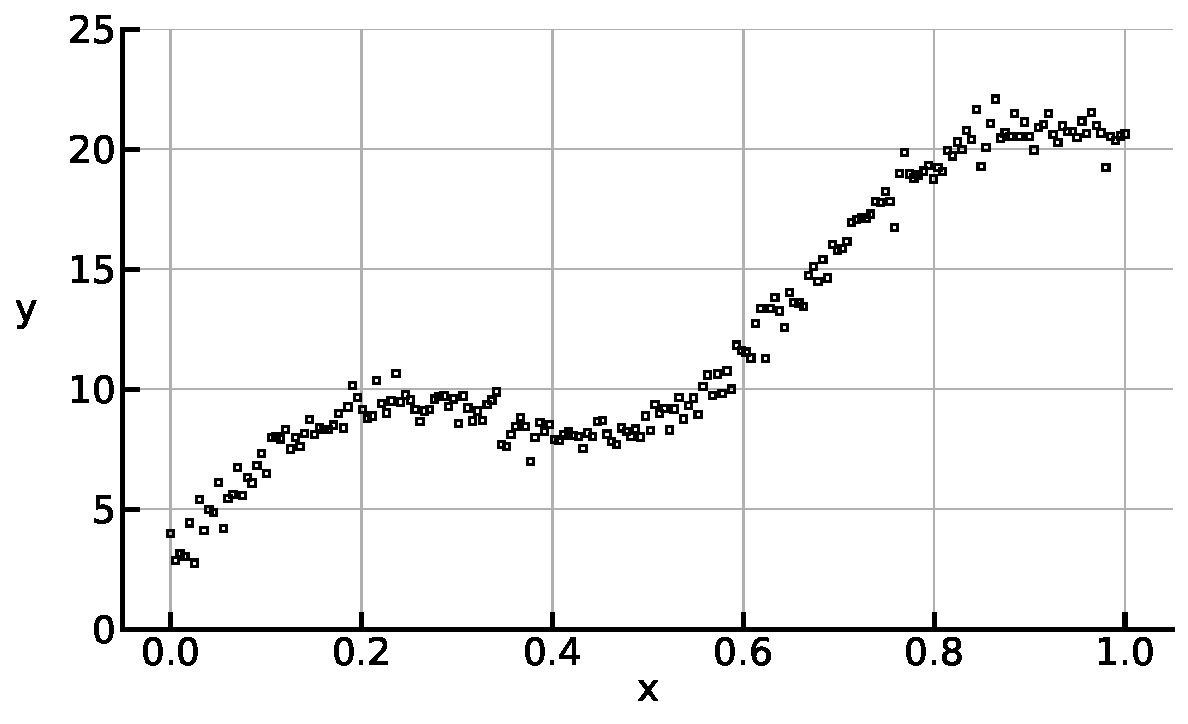
\includegraphics[width=\columnwidth]{thesisplots/test_func.pdf}
		\caption{Noisy samples determined from test function (\ref{fig:test_func})}
		\label{fig:test_func}
	\end{figure}
		Figure \ref{fig:incspline} shows an example, where the noisy data shown in Figure \ref{fig:test_func} is approximated by considering the monotonicity constraint. The estimate has to be monotonically increasing in contrast to the data, i.e. $f'(x) \ge 0$.  The smoothing parameter $\lambda_s$ was optimized using cross-validation and set to $\lambda_s=271.9$. The constraint parameter $\lambda_c$ was set to $\lambda_c = 6000$. For both function estimations, i.e. using P-splines (blue curve) vs. using constraint P-splines (red curve), the number of used splines $k$ was set to $k=30$. 	
	
	\begin{figure}[H]
	\centering
	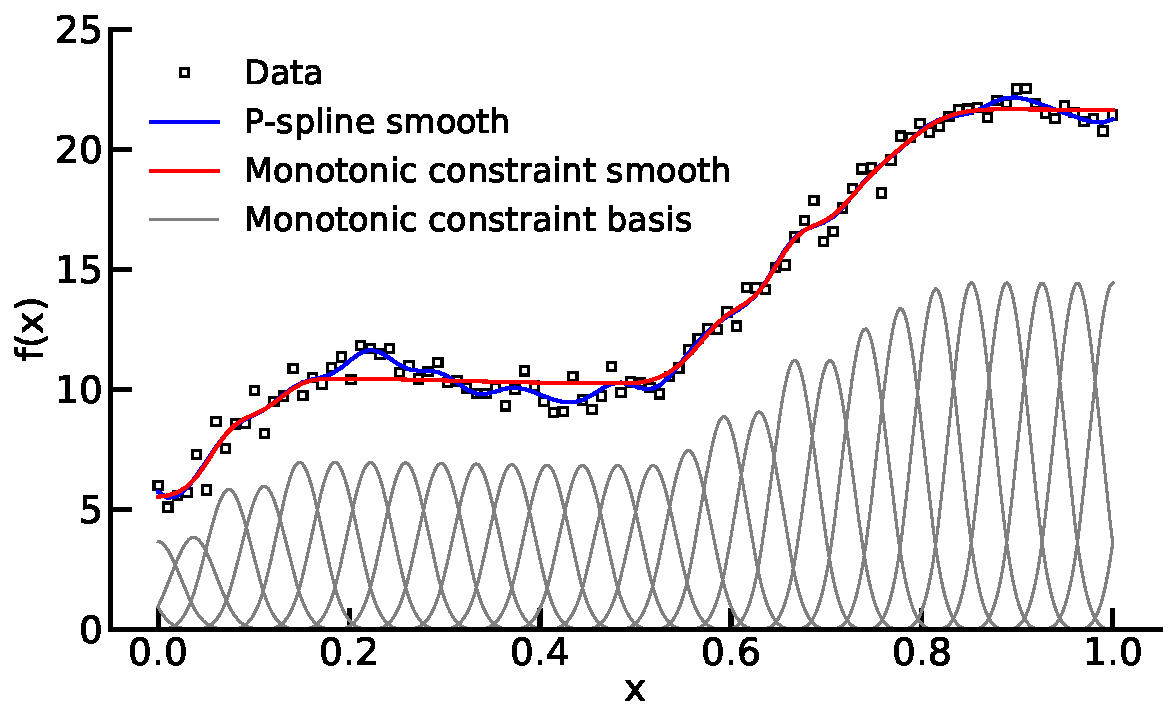
\includegraphics[width=\linewidth]{../thesisplots/inc_spline.pdf}
	\caption{Approximation of the noisy data by P-splines and P-splines with the monotonic increasing constraint}
	\label{fig:incspline}
	\end{figure}	
	
	The constraint function estimation (red curve in Figure \ref{fig:incspline}), follows the monotonicity constraint far better that the smooth function estimation (blue curve in Figure \ref{fig:incspline}). For $x < 0.15$ and $x > 0.6$, the two fits are nearly identical, since no constraint violation is present. Note, the entries of the weighting matrix $\vec{V}$ in this region are therefore $0$ because the constraint is not active. For $x \in [0.15, 0.6]$ the constraint is active. The red fit produces an almost constant line in this region as an optimal solution for the competing goals of data accuracy, smoothness and constraint fidelity.
	
	This shows, that the incorporation of a priori knowledge in the fitting process using P-splines is in principle possible using an appropriate choice of the mapping matrix $\vec{D}_c$ and the weighting matrix $\vec{V}$ as well as an iterative fitting approach using penalized iteratively reweighted least squares. These matrices are futher discussed in the following chapters.
	
	
	%%%%%%%%%%%%%%%%%%%%%%%%%%%%%%%%%%%%%%%%%%%%%%%%%%%%%%%%%%%%%%%%%%%%%%%%%%%%%%%%%%%%%%%%%%%%%%%%%%%%%%%%%%%%%%%%%
	
	
	\subsection{1d Function Estimation} \label{subsec:1d-function-estimation}
	
	The goal is to model given data
	
	\begin{align} \label{eq:data}
		\{\vec{x}, \vec{y}\} = \{x^{(i)}, y^{(i)}\}, \ i=1, 2, \dots, n 
	\end{align}
	
	using B-splines as basis functions. Therefore, we want to estimate the unknown function $\vec{y} = f(\vec{x})$, which can be represented as a linear combination of $k$ B-spline basis functions $B_j^m$ of degree $m=3$, cf. (\ref{eq:bspline-bf-approach}), as
	
	\begin{align} \label{eq:basis_function_approach}
		\vec{y} = \vec{X} \vec{\beta},
	\end{align}
	
	where $\vec{X} \in \mathbb{R}^{n\times k}$ is the B-spline basis matrix, cf. (\ref{eq:bspline-basis-matrix}), and $\vec{\beta} \in \mathbb{R}^k$ are the coefficients to be estimated. 
	
	The least squares objective function to be minimized using the complete data is then given by
	
	\begin{align} \label{eq:OF_1}
		Q_1(\vec{y}, \vec{\beta}) = \lVert \vec{y} - f(\vec{x}) \rVert^2 = \lVert \vec{y} - \vec{X}\vec{\beta} \rVert^2 
	\end{align}	
	
	The coefficients are determined ive function $Q_1$ given in (\ref{eq:OF_1}) with respect to $\vec{\beta}$, i.e.
	
	\begin{align}\label{eq:optimization_problem_1}
		\hat{\vec{\beta}}_{LS} = \arg \min_{\vec{\beta}} Q_1(\vec{y}, \vec{\beta}).
	\end{align}
	
	Using the least squares algorithm LS, see Chapter \ref{subsubsec:Method-of-LS}, the minimization problem (\ref{eq:optimization_problem_1}) yields 
	
	\begin{align} \label{eq:LS_coef}
		\hat{\vec{\beta}}_{LS}= (\transpose{\vec{X}} \vec{X})^{-1} \transpose{\vec{X}} \vec{y}.
	\end{align} 
	
	
	Figure \ref{fig:smooth_bf} shows a B-spline model using $k=10$ splines on an equidistant grid approximating the noisy data presented in Figure \ref{fig:test_func}, as well as the individual cubic ($m=3$) B-spline basis functions $B_i^3(\vec{x})$ multiplied with the corresponding, estimated coefficients $\hat{\vec{\beta}}_{LS, j} \ j=1, \dots, 10$.
	
	\begin{figure}[H]
		\centering
		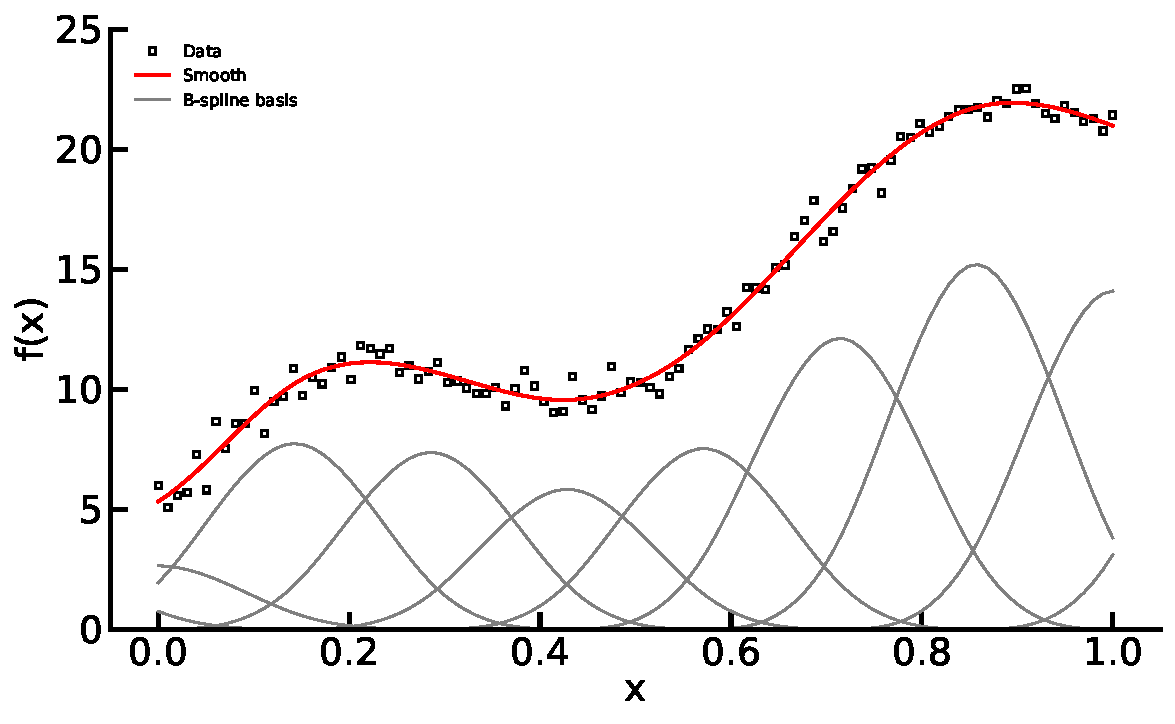
\includegraphics[width=\columnwidth]{thesisplots/smooth_bf.pdf}
		\caption{Approximation of the noisy data by B-splines without constraints}
		\label{fig:smooth_bf}
	\end{figure}
	
	
	Note, the number of splines $k$ has a strong influence on the amount of smoothing. A small number $k$ leads to a very smooth estimate, but a large data error. On the other hand, when the number of splines is relatively large, the data error is very small but the smoothness of the estimate is poor. This behavior is an example of the well-known bias-variance dilemma and depicted in Figure \ref{fig:smooth_bf_large}. \cite{sammut2011}
	Here, two B-splines models with $k=10$ and $k=50$ are illustrated, which are applied to the noisy data shown in Figure \ref{fig:test_func}. To overcome this challenges, the B-splines will be extended by penalizing the second derivative of the estimation, see Chapter \ref{subsec:1D_smooth}. 
	
	\begin{figure}[H]
		\centering
		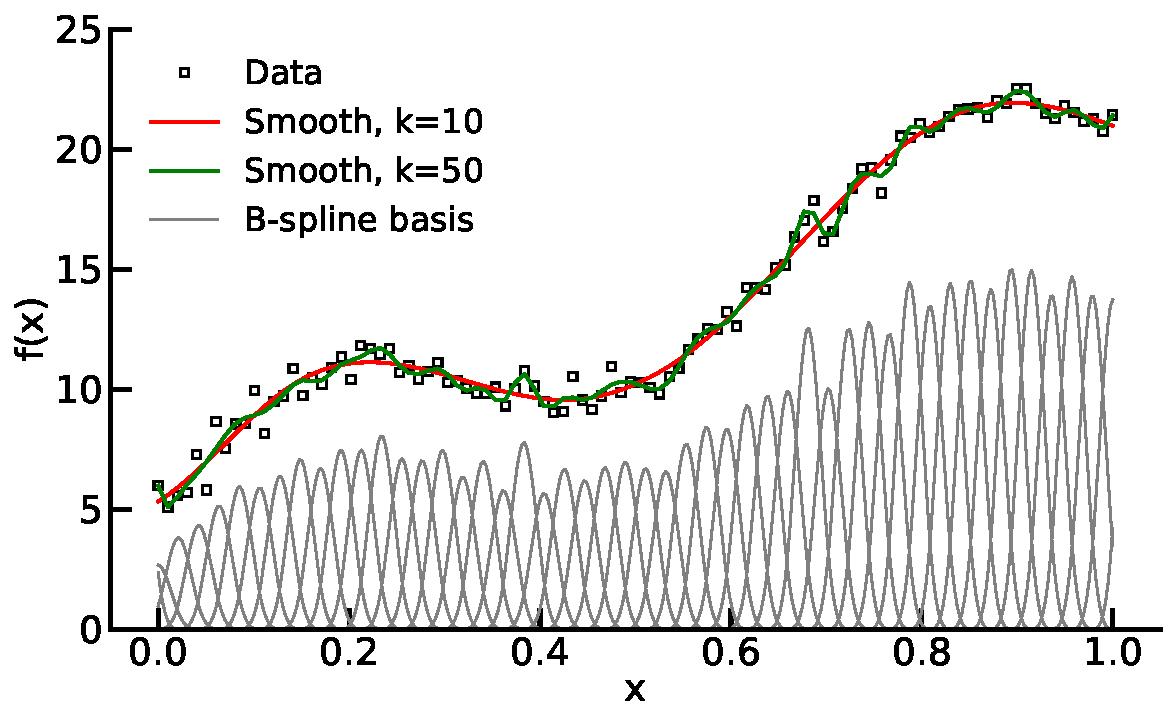
\includegraphics[width=\linewidth]{thesisplots/smooth_wiggly_bf.pdf}
		\caption{Approximation of the noisy data by 10 and 50 B-splines without constraints}
		\label{fig:smooth_bf_large}
	\end{figure}
	
	
	%%%%%%%%%%%%%%%%%%%%%%%%%%%%%%%%%%%%%%%%%%%%%%%%%%%%%%%%%%%%%%%%%%%%%%%%%%%%%%%%%%%%%%%%%%%%%%%%%%%%%%%%%%%%%%%%%
	\subsection{1d Smooth Function Estimation} \label{subsec:1D_smooth}
	
	The second derivative of the estimated function $f(x)$, i.e. $f''(x) = \sum_{j=1}^k B''_i(x) \beta_k$, has to be penalized to realize a smoother estimate when using  a high number of splines. Eilers and Marx have introduced the so-called P-splines. \cite{eilers1996flexible}, see Chapter \ref{subsec:p-splines}. Therefore, the objective function in (\ref{eq:OF_1}) is extended by an additional term considering the smoothness, i.e.
	
	\begin{align}\label{eq:OF_2}
		Q_2(\vec{y}, \vec{\beta}) = Q_1(\vec{y}, \vec{\beta}) + \lambda_s \mathcal{J}_s(\vec{\beta}; d) = \lVert \vec{y} - \vec{X} \vec{\beta} \rVert^2 + \lambda_s \transpose{\vec{\beta}} \transpose{\vec{D}}_d \vec{D}_d \vec{\beta}, 
	\end{align}
	
	with the smoothing parameter $\lambda_s$ and an appropriate mapping matrix $\vec{D}_d$ capturing the second derivative, which itself is a measure for function wiggliness. Here, an approximation of the second derivative can be performed by the squared finite difference of order $d$ of adjacent coefficients using the matrix form $\vec{D}_d$ of the difference operator of order $d$, see Chapter \ref{subsec:p-splines}. 
	
	By minimizing the objective function (\ref{eq:OF_2}), i.e.
	
	\begin{align}\label{eq:optimization_problem_2}
		\hat{\vec{\beta}}_{PLS} = \arg \min_{\vec{\beta}} Q_2(\vec{y}, \vec{\beta}),
	\end{align}
	
	using the penalized least squares algorithm PLS, the penalized least squares estimates are given by
	
	\begin{align} \label{eq:PLS_coef}
		\hat{\vec{\beta}}_{PLS}= (\transpose{\vec{X}} \vec{X} + \lambda_s \transpose{\vec{D}}_d \vec{D}_d)^{-1} \transpose{\vec{X}} \vec{y}.
	\end{align} 
	%
	In (\ref{eq:PLS_coef}), the smoothing parameter $\lambda_s$ plays a critical role and can be optimized using the information criteria specified in Chapter \ref{subsec:MAC}, e.g. AIC and BIC, or by using cross-validation techniques, see Chapter \ref{subsubsec:Cross-validation}. \cite{fahrmeir2007regression}
	
	For small values $\lambda_s \rightarrow 0$, the penalized least squares estimate $\hat{\vec{\beta}}_{PLS}$ approaches the least squares estimate $\hat{\vec{\beta}}_{LS}$, cf. (\ref{eq:LS_coef}), while for large values $\lambda_s \gg 0$, the fitted function shows the behavior of a polynomial with $d-1$ degrees of freedom. For example, using $d=2$ and a large smoothing parameter $\lambda_s$ this configuration leads to a linear function, while using $d=1$ would lead to a constant function. \cite{fahrmeir2007regression}
	
	Figure \ref{fig:psplines} shows the behavior of P-splines of degree $m=3$ using $k=50$ splines for several values of the smoothing parameter $\lambda_s = \{10^{-2}, 10^{2},10^{5},10^{6}\}$ and a smoothness penalty of order $d=2$.  As the value of $\lambda_s$ gets larger, the fitted curve becomes more smooth and thus the $2^{nd}$ derivative of the curve becomes smaller due to the penalty considered in the estimation, see (\ref{eq:PLS_coef}). For very large values of $\lambda_s$, the estimate approaches a straight line, see the yellow curve in Figure \ref{fig:psplines}.
	
	\begin{figure}[H]
		\centering
		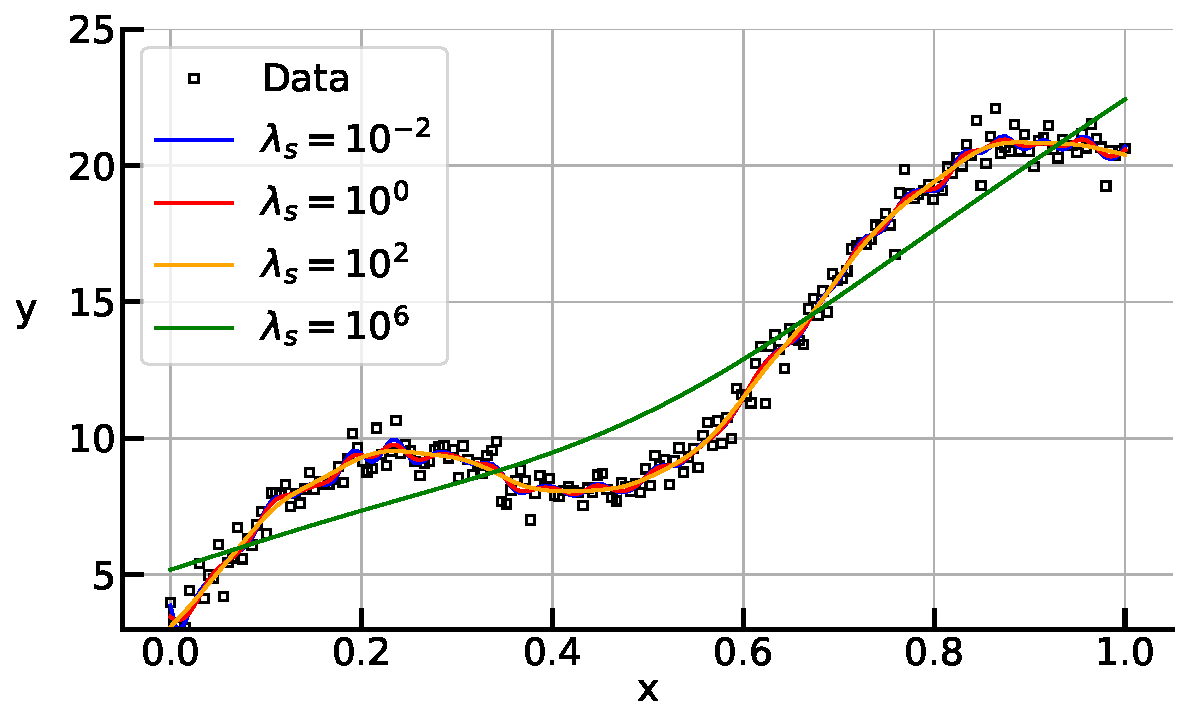
\includegraphics[width=\linewidth]{thesisplots/p_splines.pdf}
		\caption{Smooth function estimation for different smoothing parameters $\lambda_s$}
		\label{fig:psplines}
	\end{figure}
	
	%%%%%%%%%%%%%%%%%%%%%%%%%%%%%%%%%%%%%%%%%%%%%%%%%%%%%%%%%%%%%%%%%%%%%%%%%%%%%%%%%%%%%%%%%%%%%%%%%%%%%%%%%%%%%%%%%
	\subsection{1d Constraint Function Estimation}
	%%%%%%%%%%%%%%%%%%%%%%%%%%%%%%%%%%%%%%%%%%%%%%%%%%%%%%%%%%%%%%%%%%%%%%%%%%%%%%%%%%%%%%%%%%%%%%%%%%%%%%%%%%%%%%%%%
	%%%%%%%%%%%%%%%%%%%%%%%%%%%%%%%%%%%%%%%%%%%%%%%%%%%%%%%%%%%%%%%%%%%%%%%%%%%%%%%%%%%%%%%%%%%%%%%%%%%%%%%%%%%%%%%%%	
	\section{User-defined Constraints} \label{sec:user-defined-constraints}
	
	As stated before, a priori domain knowledge given in Table \ref{tab:constraint_overview} can be introduced by the choice of the mapping matrix $\vec{D}_c$ and the weighting matrix $\vec{V}$, cf. (\ref{eq:mapping_matrix}) and (\ref{eq:PLS,c_coef}). Now a description of the different matrices, which are used to enforce the a priori known domain behavior, is presented. 
	
	%%%%%%%%%%%%%%%%%%%%%%%%%%%%%%%%%%%%%%%%%%%%%%%%%%%%%%%%%%%%%%%%%%%%%%%%%%%%%%%%%%%%%%%%%%%%%%%%%%%%%%%%%%%%%%%%%
	\subsection{Monotonicity Constraint}
	
	The mapping matrix $\vec{D}_{monoton}$ enforcing monotonic behavior is given by the first order difference operator $\Delta^1$ for equidistant knot placement, cf. \ref{eq:d1-difference-matrix}. The corresponding matrix for $k$ splines is given as
	
	\begin{align} \label{eq:D_c_monoton}
		\vec{D}_{monoton} = \begin{pmatrix}  -1 & 1  &  		& \\ 
			& -1 & 1 		& \\ 
			&    & \ddots  & \ddots  
		\end{pmatrix} \in \mathbb{R}^{k-1 \times k}.
	\end{align}
	
	The difference between monotonic increasing and decreasing behavior is controlled by the weighting matrix $\vec{V}$. For increasing behavior, the weighting matrix $\vec{V}$ is given by the weights $v_j$ according to
	
	\begin{align} \label{eq:v_monoton_inc}
		v_j(\vec{\beta}) = \begin{cases}
			0, \quad \text{if} \ \Delta^1\beta_j \ge 0 \\ 
			1, \quad \text{if} \ \Delta^1\beta_j < 0
		\end{cases}	\ \text{for} \ j=2, \dots, k-1.
	\end{align}
	
	For decreasing behavior, the weighting matrix $\vec{V}$ is given by the weights $v_j$ according to
	\begin{align} \label{eq:v_monoton_dec}
		v_j(\vec{\beta}) = \begin{cases} 0, \quad \text{if} \ \Delta^1\beta_j \le 0 \\ 
			1, \quad \text{if} \ \Delta^1\beta_j > 0
		\end{cases} \ \text{for} \ j=2, \dots, k-1.
	\end{align}
	
	This states, that the penalty term $\mathcal{J}_c(\vec{\beta}; c)$ only contributes if adjacent coefficients $\beta_{j-1}$ and $\beta_j$ are increasing or decreasing, respectively. \cite{hofner2011monotonicity} \cite{eilers2005unimodal}
	
	%%%%%%%%%%%%%%%%%%%%%%%%%%%%%%%%%%%%%%%%%%%%%%%%%%%%%%%%%%%%%%%%%%%%%%%%%%%%%%%%%%%%%%%%%%%%%%%%%%%%%%%%%%%%%%%%%	
	\subsection{Curvature Constraint}
	
	In the simplest case, the curvature of the function $f(x)$ can either be convex, i.e. $f''(x) \ge 0$, or concave, i.e. $f''(x) \le 0$. The mapping matrix $\vec{D}_{curvature}$ enforcing this behavior can be approximated by the second order difference operator $\Delta^2$ for equidistant knot placement, cf. (\ref{eq:d2-difference-matrix}). The corresponding matrix for $k$ splines is given as
	
	\begin{align} \label{eq:D_c_curvature}
		\vec{D}_{curvature} = \begin{pmatrix} 1 & -2 & 1 		&  		 & \\ 
			& 1  &-2 	    &1 		 & \\
			& 	  & \ddots  & \ddots & \ddots  
		\end{pmatrix} \in \mathbb{R}^{k-2 \times k}.
	\end{align}	
	
	The difference between concave and convex curvature is controlled by the weighting matrix $\vec{V}$. For concave curvature, the weighting matrix $\vec{V}$ is given by the weights $v_j$ according to
	
	\begin{align}\label{eq:v_curvature_concave}
		v_j(\vec{\beta}) = \begin{cases} 
			0, \quad \text{if} \ \Delta^2\beta_j \le 0 \\ 
			1, \quad \text{if} \ \Delta^2\beta_j > 0
		\end{cases} \ \text{for} \ j=1, \dots, k-2.
	\end{align}
	
	For convex curvature, the weighting matrix $\vec{V}$ is given by the weights $v_j$ according to
	
	\begin{align}\label{eq:v_curvature_convex}
		v_j(\vec{\beta}) = \begin{cases} 
			0, \quad \text{if} \ \Delta^2\beta_j \ge 0 \\ 
			1, \quad \text{if} \ \Delta^2\beta_j < 0
		\end{cases}\ \text{for} \ j=1, \dots, k-2.
	\end{align}	
	
	Therefore, the penalty term $\mathcal{J}_c(\vec{\beta}; c)$ in (\ref{eq:OF_3}) or (\ref{eq:PLS,c_coef}) only contributes if the second order difference of adjacent coefficients $\vec{\beta}$ is either positive or negative, respectively. \cite{eilers2005unimodal}
	
	%%%%%%%%%%%%%%%%%%%%%%%%%%%%%%%%%%%%%%%%%%%%%%%%%%%%%%%%%%%%%%%%%%%%%%%%%%%%%%%%%%%%%%%%%%%%%%%%%%%%%%%%%%%%%%%%%	
	\subsection{Unimodality Constraint}

	%%%%%%%%%%%%%%%%%%%%%%%%%%%%%%%%%%%%%%%%%%%%%%%%%%%%%%%%%%%%%%%%%%%%%%%%%%%%%%%%%%%%%%%%%%%%%%%%%%%%%%%%%%%%%%%%
	\subsection{Boundedness Constraint}

	%%%%%%%%%%%%%%%%%%%%%%%%%%%%%%%%%%%%%%%%%%%%%%%%%%%%%%%%%%%%%%%%%%%%%%%%%%%%%%%%%%%%%%%%%%%%%%%%%%%%%%%%%%%%%%%%
	\subsection{Jamming Constraint}
	

	
	%%%%%%%%%%%%%%%%%%%%%%%%%%%%%%%%%%%%%%%%%%%%%%%%%%%%%%%%%%%%%%%%%%%%%%%%%%%%%%%%%%%%%%%%%%%%%%%%%%%%%%%%%%%%%%%%
	\subsection{Penalty Term for Tensor-Product Splines}
	
	To extend the framework of mapping matrices to two dimensions and tensor-product splines, we again use the concept of Kronecker products given in Chapter \ref{subsubsec:tp-splines}. In principle, every possible pair of one dimensional user-defined constraints can be constructed using the approach in Chapter \ref{subsubsec:tp-splines}, e.g. unimodality in two dimensions would be obtained using the unimodal mapping matrix depicted above for each dimension. We then also need to include the constraint specific weight matrices $\vec{V}$.
	
	The penalty term for the constraint given by $c_1$ for dimension $1$ and $c_2$ for dimension $2$ then has the form
	
	\begin{align} \label{eq:J-c-tps}
		\mathcal{J}_c(\vec{\beta}; c) = \transpose{\vec{\beta}} \Big[ \vec{I}^2 \otimes \vec{K}_{c_1} + \vec{K}_{c_2} \otimes \vec{I}^1\Big] \vec{\beta}
	\end{align}
	
	with the respective penalty matrices $\vec{K}_{c_1} = \vec{D}_{c_1}^{\text{T}} \vec{V}_1 \vec{D}_{c_1}$ for dimension $x_1$ and $\vec{K}_{c_2} = \vec{D}_{c_2}^{\text{T}} \vec{V}_2 \vec{D}_{c_2}$ for dimension $x_2$ using the weighting matrices $\vec{V}_1$ and $\vec{V}_2$, the mapping matrices $\vec{D}_{c_1}$ and $\vec{D}_{c_2}$ and the identity matrices $\vec{I}^1$ and $\vec{I}^2$ for the respective dimension.
	
	%%%%%%%%%%%%%%%%%%%%%%%%%%%%%%%%%%%%%%%%%%%%%%%%%%%%%%%%%%%%%%%%%%%%%%%%%%%%%%%%%%%%%%%%%%%%%%%%%%%%%%%%%%%%%%%%%
	%%%%%%%%%%%%%%%%%%%%%%%%%%%%%%%%%%%%%%%%%%%%%%%%%%%%%%%%%%%%%%%%%%%%%%%%%%%%%%%%%%%%%%%%%%%%%%%%%%%%%%%%%%%%%%%%%
	\section{n-d Constraint Function Estimation}
	
	The extension from one input to multiple input dimensions uses the concept of additive models given in Chapter \ref{subsubsec:STAR}. Given input data $\{ x_1^{(i)}, \dots, x_q^{(i)}, y^{(i)}\}, \ i=1, 2, \dots, n$ and $q$ as the number of inputs, the combined model using all available B-splines and tensor-product splines is given, cf. (\ref{eq:STAR}), as
	
	\begin{align} \label{eq:tps_all}
		y = f(x_1,..., x_q) = \sum_{j=1}^q s_j(x_j) + \sum_{j=1}^{q-1} \sum_{r>j}^q t_{j, r}(x_j, x_r)
	\end{align}
	
	where $s_j(x_j)$ is the B-spline estimate given by $s_j(x_j) = \vec{X}_{s_j} \vec{\beta}_{s_j}$ and $t_{j, r}(x_j,x_r)$ is the tensor-product estimate is given by $t_{j, r}(x_j,x_r) = \vec{X}_{t_{j,r}} \vec{\beta}_{t_{j, r}}$. The number of individual estimates is given by 
	
	\begin{align}
		n_{total} = q + \frac{q(q-1)}{2}.  
	\end{align}
	
	The constrained penalized least squares objective function for additive models can now be written similar to (\ref{eq:OF_3}) as
	
	\begin{align}\label{eq:OF_6}
		Q_6(\vec{y}, \vec{\beta}) = Q_1(\vec{y}, \vec{\beta}) + \transpose{\vec{\lambda}}_s	\vec{\mathcal{J}}_s(\vec{\beta}; \vec{d}) + \transpose{\vec{\lambda}}_c \vec{\mathcal{J}}_c(\vec{\beta}; \vec{c}).
	\end{align}
	
	with $\vec{\lambda}_s \in \mathbb{R}^{n_{total}}$ and  $\vec{\lambda}_c \in \mathbb{R}^{n_{total}}$  defined as vectors with one value of smoothness and constraint parameter for each individual estimate, respectively. 
	
	We now need to specify the three parts of the objective function in (\ref{eq:OF_6}). 
	
	%%%%%%%%%%%%%%%%%%%%%%%%%%%%%%%%%%%%%%%%%%%%%%%%%%%%%%%%%%%%%%%%%%%%%%%%%%%%%%%%%%%%%%%%%%%%%%%%%%%%%%%%%%%%%%%%%
	\subsection{Data Term}
	
	Assuming the use of $k$ splines for the B-spline estimates and $k^2$ splines for the tensor-product estimates, the total number of coefficients to be determined is given by 
	
	\begin{align}\label{eq:tps_total_number_of_coef}
		k_{total} = qk + \frac{q(q-1)}{2}k^2. 
	\end{align}
	
	Since all B-spline and tensor-product spline models follow a linear model structure, see Chapter \ref{subsec:b-splines} and \ref{subsubsec:tp-splines}, we can combine them into one large model, cf. (\ref{eq:STAR-block-diag}), given by
	
	\begin{align}\label{eq:tps_lin_mod}
		\vec{y} = \vec{X} \vec{\beta}
	\end{align}
	
	where the matrix $\vec{X} \in \mathbb{R}^{n \times k_{total}}$ is given in (\ref{eq:STAR-block-diag}) as horizontal concatenation of the individual bases and the combined coefficient vector $\vec{\beta} \in \mathbb{R}^{k_{total}}$ is given in (\ref{eq:STAR-block-diag}) by a vertical concatenation of the individual coefficient vectors. 
	
	The data term $Q_1(\vec{y}, \vec{\beta})$ in the constrained penalized least squares objective function given in (\ref{eq:OF_6}) can now be evaluated using arbitrary input dimensions. 
	
	%%%%%%%%%%%%%%%%%%%%%%%%%%%%%%%%%%%%%%%%%%%%%%%%%%%%%%%%%%%%%%%%%%%%%%%%%%%%%%%%%%%%%%%%%%%%%%%%%%%%%%%%%%%%%%%%%
	\subsection{Smoothness Term}
	
	The combined smoothness penalty term $\vec{\mathcal{J}}_s(\vec{\beta}; \vec{d}) \in \mathbb{R}^{n_{total}}$ is then given as
	
	\begin{align}\label{eq:J_s_ndim}
		\vec{\mathcal{J}}_s(\vec{\beta}; \vec{d}) &= 
		\begin{pmatrix}
			\mathcal J_{s_1}(\vec{\beta}_{s_1}; d_{s_1}) \\ 
			\vdots \\ 
			\mathcal J_{s_q}(\vec{\beta}_{s_q}; d_{s_q}) \\
			\mathcal J_{t_{1,2}}(\vec{\beta}_{t_{1,2}}; d_{t_{1,2}}) \\
			\vdots \\
			\mathcal J_{t_{q-1,q}}(\vec{\beta}_{t_{q-1,q}}; d_{t_{q-1,q}}) \\
		\end{pmatrix}
	\end{align}
	
	with $\mathcal J_e(\vec{\beta}_e; d_e) = \transpose{\vec{\beta}}_e \transpose{\vec{D}}_{d_e} \vec{D}_{d_e} \vec{\beta}_e$ determining the smoothness penalty term using the coefficients $\vec{\beta}_e$ and mapping matrix $\vec{D}_{d_e}$, see Chapter \ref{subsec:p-splines} and Chapter \ref{subsubsec:tp-splines}, for each estimate $e \in \{s_1, \dots, s_q, t_{1,2}, \dots, t_{q-1,q}\}$. The vector $\vec{d} \in \mathbb{R}^{n_{total}}$ consists of the orders $d_e$ determining the mapping matrix $\vec{D}_{d_e}$ of the smoothness constraint for each individual estimate $e$. 
	
	%%%%%%%%%%%%%%%%%%%%%%%%%%%%%%%%%%%%%%%%%%%%%%%%%%%%%%%%%%%%%%%%%%%%%%%%%%%%%%%%%%%%%%%%%%%%%%%%%%%%%%%%%%%%%%%%%
	\subsection{Constraint Term}
	The combined constraint penalty term $\vec{\mathcal{J}}_c(\vec{\beta}; \vec{c}) \in \mathbb{R}^{n_{total}}$ is then given as
	
	\begin{align}\label{eq:J_c_ndim}
		\vec{\mathcal{J}}_c(\vec{\beta}; \vec{c}) &= 
		\begin{pmatrix}
			\mathcal J_{s_1}(\vec{\beta}_{s_1}; c_{s_1}) \\ 
			\vdots \\ 
			\mathcal J_{s_q}(\vec{\beta}_{s_q}; c_{s_q}) \\
			\mathcal J_{t_{1,2}}(\vec{\beta}_{t_{1,2}}; c_{t_{1,2}}) \\
			\vdots \\
			\mathcal J_{t_{q-1,q}}(\vec{\beta}_{t_{q-1,q}}; c_{t_{q-1,q}}) \\
		\end{pmatrix}
	\end{align}
	
	with $\mathcal J_e(\vec{\beta}_e; c_e) = \transpose{\vec{\beta}}_e \transpose{\vec{D}}_{c_e} \vec{V}_{c_e} \vec{D}_{c_e} \vec{\beta}_e$ determining the constraint penalty term using the coefficients $\vec{\beta}_e$, the mapping matrix $\vec{D}_{c_e}$ and the weighting matrix $\vec{V}_e$ for each estimate $e \in \{s_1, \dots, s_q, t_{1,2}, \dots, t_{q-1,q}\}$, see Chapter (\ref{sec:user-defined-constraints}). The vector $\vec{c} \in \mathbb{R}^{n_{total}}$ consists of the constraint type $c_e$, e.g. monoton increasing, determining the mapping matrix $\vec{D}_{c_e}$ for each individual estimate $e$. 
	
	%%%%%%%%%%%%%%%%%%%%%%%%%%%%%%%%%%%%%%%%%%%%%%%%%%%%%%%%%%%%%%%%%%%%%%%%%%%%%%%%%%%%%%%%%%%%%%%%%%%%%%%%%%%%%%%%%
	
	The objective function (\ref{eq:OF_6}) is then optimized, i.e.
	
	\begin{align}\label{eq:optimization_problem_6}
		\hat{\vec{\beta}}_{PLS,c,nd} = \arg \min_{\vec{\beta}} Q_6(\vec{y}, \vec{\beta}),
	\end{align}
	
	using the penalized iteratively reweighted least squares algorithm, cf. (\ref{eq:PLS,c_coef}), to obtain the coefficients $\hat{\vec{\beta}}_{PLS,c,nd}$ as
	
	\begin{align} \label{eq:beta-pls-c-nd-formula}
		\hat{\vec{\beta}}_{PLS,c,nd} = (\transpose{\vec{X}} \vec{X} +\vec{K}_s + \vec{K}_c)^{-1} \transpose{\vec{X}} \vec{y}. 
	\end{align}
	
	In (\ref{eq:beta-pls-c-nd-formula}), $\vec{X} \in \mathbb{R}^{n \times k_{total}}$ is the combined basis matrix, cf. (\ref{eq:STAR-block-diag}), $\vec{K}_s \in \mathbb{R}^{k_{total} \times k_{total}}$ is the combined smoothness matrix given as
	
	\begin{align} \label{eq:combined-smoothness-matrix}
		\vec{K}_s = \rotatebox{-90}{$\begin{pmatrix} 
				\lambda_{s_1} \transpose{\vec{D}_{d_{s_1}}} \vec{D}_{d_{s_1}} & 0 \\
				0 						  &	\ddots & 0 \\
				&  0 	   & \lambda_{s_q} \transpose{\vec{D}_{d_{s_q}}} \vec{D}_{d_{s_q}} & 0 \\
				&        &           0										   & \lambda_{s_{1,2}} \transpose{\vec{D}_{d_{t_{1,2}}}} \vec{D}_{d_{t_{1,2}}} & 0 \\
				&  & &    0 & \ddots & 0 \\
				&  & &      &   0    & \lambda_{s_{q-1,q}} \transpose{\vec{D}_{d_{t_{q-1,q}}}} \vec{D}_{d_{t_{q-1,q}}}
			\end{pmatrix}$} 
	\end{align}
	
	and $\vec{K}_c \in \mathbb{R}^{k_{total} \times k_{total}}$ is the combined constraint matrix as 
	
	\begin{align} \label{eq:combined-constraint-matrix}
		\vec{K}_c = \rotatebox{-90}{$\begin{pmatrix} 
				\lambda_{c_1} \transpose{\vec{D}_{c_{s_1}}} \vec{V}_{c_{s_1}} \vec{D}_{c_{s_1}} & 0 \\
				0 						& \ddots & 0 \\
				&  0 	 & \lambda_{c_q} \transpose{\vec{D}_{c_{s_q}}} \vec{V}_{c_{s_q}} \vec{D}_{c_{s_q}} & 0 \\
				&        &           0										    & \lambda_{c_{1,2}} \transpose{\vec{D}_{c_{t_{1,2}}}} \vec{V}_{c_{t_{1,2}}} \vec{D}_{c_{t_{1,2}}} & 0 \\
				& &  &   0 & \ddots & 0 \\
				& &  & 	   &	0   & \lambda_{c_{q-1,q}} \transpose{\vec{D}_{c_{t_{q-1,q}}}} \vec{V}_{c_{t_{q-1,q}}} \vec{D}_{c_{t_{q-1,q}}}
			\end{pmatrix}$}. 
	\end{align}
	
	
	
	
	%%%%%%%%%%%%%%%%%%%%%%%%%%%%%%%%%%%%%%%%%%%%%%%%%%%%%%%%%%%%%%%%%%%%%%%%%%%%%%%%%%%%%%%%%%%%%%%%%%%%%%%%%%%%%%%%%%%
	\subsection{2-d Example} \label{subsec:2d-example}
	
	As example for the n-d constraint function estimation, we take a look at the function 
	
	\begin{align} \label{eq:2d_test_func}
		f(x_1, x_2) = 2\exp{\Big(-\frac{(x_1 - 0.25)^2}{0.08}\Big)} + x_2^2 + \eta
	\end{align}
	
	for $x_1 \in [0,1]$ and $x_2 \in [0,1]$ and random Gaussian noise $\eta$ with $\sigma_{noise} = 0.1$. Therefore we expect a peak in dimension $x_1$ as well as increasing behavior for dimension $x_2$, see Figure \ref{fig:2d_example}. The user-defined constraints are therefore $c_1 = \text{unimodal}$ and $c_2 = \text{monotonic increasing}$ Using this knowledge, we create a model with the following characteristics:
	
	\begin{itemize}
		\item B-spline smooth $s_1(x_1)$: $k_{x_1} = 50$, $c = c_1$, $\lambda_s = 1$ and $\lambda_c = 6000$
		\item B-spline smooth $s_2(x_2)$: $k_{x_2} = 50$, $c = c_2$, $\lambda_s = 1$ and $\lambda_c = 6000$
	\end{itemize}
	
	The fit for this model as well as the individual estimates $s_1(x_1)$ and $s_2(x_2)$ are shown in Figure \ref{fig:2d_example}. The model fits the data quite well and holds the specified constraints for the individual dimensions.
	
	\begin{figure}[H]
		\centering
		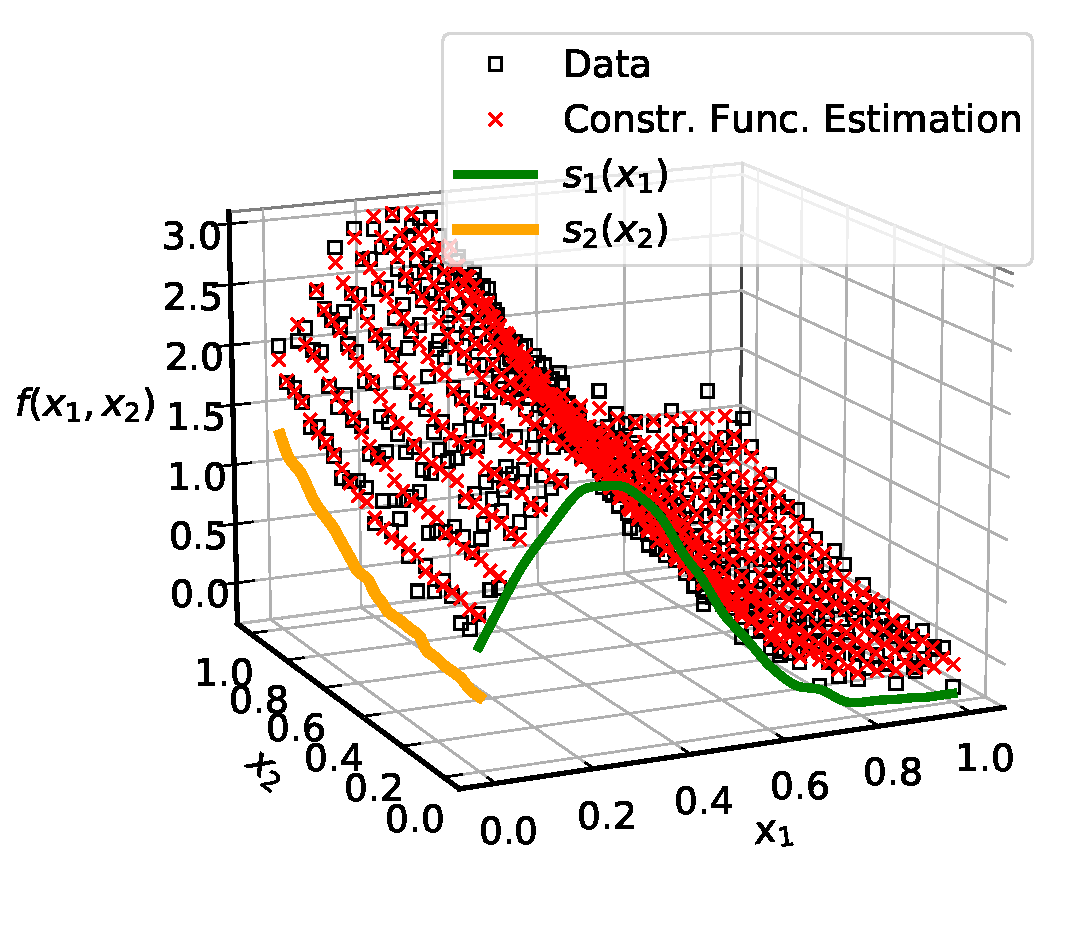
\includegraphics[width=\linewidth]{thesisplots/2d_example.pdf}
		\caption{2-d test function for n-d constrained function estimation}
		\label{fig:2d_example}
	\end{figure}
	
\end{comment}

%%%%%%%%%%%%%%%%%%%%%%%%%%%%%%%%%%%%%%%%%%%%%%%%%%%%%%%%%%%%%%%%%%%%%%%%%%%%%%%%%%%%%%%%%%%%%%%%%%%%%%%%%%%%%%%%%%%%%%%%%%%%%%%%%%%%%%%%%%%%%%%%%%%%%%%%%%%%%%%%%%%%%%%%%%%%%%%%%%%%%%%%%%%%%%%%%%%%%%%%%%%%%%%%%%%%%%%%%%%%%%%%%%%%%%

\bibliographystyle{IEEEtran}
\bibliography{../bibliography}
			  
%\printbibliography


\end{document}